\documentclass{maine-thesis}  % Default options 12pt and final copy

% Include necessary packages here
% \usepackage{...}

% Replace contents of {...} with your own information.
\title{...}					% Title of thesis
\author{...}					% Author's name: First Middle Last
\degreesheld{...}			% Previously earned degree(s), institution(s) and year(s).  
\degree{...}  				% Degree to be granted
\program{...}				% Degree granting department or program
\submitdate{...}				% Month and year of graduation (do not separate with a comma)

\principaladvisor{...} 			% Advisors name, title
% If you have more than one advisor then you'll also need the following command, otherwise comment out or delete it
\secondadvisor{...}

% Include all committee members names and titles
\firstreader{...}        
\secondreader{...}
% If necessary (i.e. for a doctorate), include extra committee members.  Else, comment out or delete any that are unnecessary
\thirdreader{...}
\fourthreader{...}
\fifthreader{...}

\principalshort{...} 			% Shortened advisor name for abstract.  See guidelines for example.
								 
% If the thesis has MORE than one appendix, leave the following command in.  Else, comment it out.
\multipleappendicestrue 

% Begin the document.
\begin{document}
\preliminary
\titlepage

% !TEX root =  Main.tex
%\preparetocs
\dissacceptance
\copyrightpage[<Copyright holder appears here, see Section \ref{copy} for details>]{<Copyright year appears here>}
\libraryrights

\begin{abstract}
The abstract for you thesis will appear on this page.  It should be limited to 350 words for a Ph.D thesis or 500 words for a Master's thesis.
\end{abstract}

\begin{layabstract}{Lay abstract keywords appear here}
The Grad School now requires a lay abstract of up to 350 words for all theses, but also requires that the lay abstract be submitted electronically to Cyrstal Burgess (email: \verb=crystal.burgess@maine.edu=).  Whether you include it in the bound version of your thesis is your choice.

If you do want to include the lay abstract in the bound version of your thesis then it will appear here.
\end{layabstract}

\begin{preface}
\section{Preface from the 2003 version}

 This class file is written for use with the \LaTeXe\ document preparation system for theses
 conforming to the guidelines of the Graduate School at the University of Maine.  
 Ideas for this class were found in  
 the class files \verb=gt-thesis.cls=\footnote{available at
 http://www.ctan.org} and \verb=rpithesis.cls=.\footnote{can be currently found at
  http://www.rpi.edu/computing/software/latex/thesis-info.html}  This class
 file is relatively compact, without too many options for the user.  A majority of the
 credit for this class should go to the original writers of those two classes.  

 \paragraph{What This Class File Can Do---}
 \verb=maine-thesis.cls= can format a masters or doctoral thesis according to the guidelines set
 forth by the Graduate School of the University of Maine.  It produces a double spaced, one sided
 document with the correct margins for final publication. 
 It will properly format a titlepage, 
 optional copyright page, abstract, optional dedication, acknowledgements and preface sections,
 a table of contents, lists of tables and figures, main matter, and end matter.  The Graduate
 School is relatively lenient in some formatting issues and strict in others.  Where there is
 leniency, decisions were made that I thought looked best.  Changes can be made to the class file
 to make it look more to your liking, but in its current version, this class file
 will produce a thesis that is acceptable to the Graduate School.
 \paragraph{A Final Note---}
 A word of warning:  {\bfseries THE GUIDELINES OF THE GRADUATE SCHOOL CAN AND DO CHANGE.}	
 This class was written using the most recent set of guidelines [...]\footnote{Date of the guidelines used by the original package author has been removed to avoid confusion.}.  
 They do change every so often so be sure that you have a copy of the most recent set of
 guidelines.  Most changes that are made will probably be small and cosmetic but there is no guarantee that
 something major will not arise.  
 
 \begin{flushright}
 Jim Kenneally
 \end{flushright}
 
\section{Preface to version 1.5}
As Jim predicted, the guidelines of the graduate school have changed a bit over the years since he originally designed this class file.  Over those intervening years every successive person who has used the class file has been required by the Graduate School to make some changes: some in response to things which Jim didn't get quite right, most to things which they had changed or become stricter on.  In most cases those changes accumulated in various versions of the file and were handed on to the next person interested in using the class file.  In some cases, however, a student would leave before they handed the class file on to anyone and as a result any changes they made would be lost and have to be reproduced.

I've made the effort to acquire all versions of the class file that I can and to consolidate the changes they contain into a single project.  I've also requested feedback from the Graduate School to make sure that this package conforms to their current standards.  This is the result.  I hope you find it useful and easy to use.

If the Graduate School requires you to change some aspect of your thesis formatting which you believe should be taken care of by this class file, please email me (\email) with a detailed description of the problem and a simple sample document that reproduces it (I don't want your whole thesis, just the part that's not right).  While I cannot guarantee that I will get to it right away, I will look at the problem just as soon as I have time and will endeavor to fix it.  If you can't afford to wait for me to fix the problem and find a fix that works, please email me that fix as well, as it's much easier for me to incorporate a fix than it is to diagnose and fix a problem.

As of April 2016, this thesis class is now hosted on GitHub (\url{https://github.com/rpspringuel/maine-thesis}).  If you have a GitHub account (they are free), you can submit Issues (bug reports) and Pull Requests (suggested changes) there.

\begin{flushright}
R. Padraic Springuel\\
Most recent version of Graduate School guidelines used: June 2015\\
Documentation last edited on \today
\end{flushright}

\end{preface}

\begin{dedication}
Dedications are optional, but if you have one it will appear here.
\end{dedication}

\begin{acknowledgements}
While acknowledgements are technically optional, they are also the perfect place to make note of funding sources, collaborators, and other people whose work made your thesis possible.  This is also the place to mention an External Reader (i.e. some one from outside the University who read and commented on your thesis) if you have one.  Acknowledgements appear here.
\end{acknowledgements}

\tableofcontents
\listoftables
\listoffigures

\begin{listof}{Whatever}
If you have some an consistent set of theorems, symbols, abbreviations, or definitions, then you must include a page which lists them just as you list the tables and figures in your thesis.
\end{listof}

\mainmatter{bottom}

\endinput

% Main text of the thesis.  Use of the `\input' command will make later editing much easier.
% !TEX root =  Main.tex
\chapter{Introduction}
This file serves both as documentation for the maine-thesis.cls and as an example of its use.  Indeed, you probably noticed this as you started paging through the first few pages in order to get to the actual documentation.  For that, I apologize, but the dual nature of this document made it necessary for all those pages to come first, seeing as that's where the Graduate School requires them to be.

This document is not intended to be an introduction on how to use \LaTeX. In fact, I will assume that you are familiar with basic \LaTeX\ commands and have typeset documents in \LaTeX\ before throughout this document.  If you haven't, then I highly suggest finding a reference book or tutorial that will teach you the basics of \LaTeX\ and read through that first.  There are several options available both in print and online (e.g. \cite{Kopka:2004,Mittelbach:2004,Flynn:2005}).  Which one you use is largely a matter of preference.

\section{Installation}
To install this class file you need to place it in \verb=~=/texmf/tex/latex/ where the ``\verb=~='' represents the location of your local texmf directory.\footnote{The final path should not have .../texmf/texmf/... in it, just .../texmf/...}  Since this changes from system to system, I can't be more specific than that, so check the documentation for your system.

\section{Organizing your Thesis}
While not required by the class file, I have some specific recommendations as to how you should organize the tex files that make up your thesis.  These recommendations are designed to make editing and distribution of drafts easier and were followed in assembling this document.  While I will go into more detail about this structure as I go over the various elements of the maine-thesis.cls file and how to use them, the basic message is to break the thesis up into multiple files.  In particular, the break down that I use is:
\begin{description}
\item[Main.tex] This file has the responsibility for coordinating all the other files, but contains very little of the actual body of the thesis.
\item[Front.tex] This file contains all the material which appears up to and including the Table of Contents.
\item[Ch\#.tex] The individual chapters of your thesis.  By splitting out each thesis chapter into its own file, it will be easier to find where you want to work in any particular session as well as make generating draft copies of just part of the thesis easier.
\item[App\#.tex] Like the chapter files, each appendix gets its own file.
\item[Biography.tex] The last element of the thesis, the biography of the author also gets its own file to avoid adding clutter to Main.tex.
\item[Figures] Since most of the figures you use in your thesis are likely to be separate image files which \LaTeX\ will need access to when it typesets your thesis, I advise making a subfolder for your project where you can place these images.  It'll make them easier to find later when you need to change them and keep the project root folder from getting too cluttered.
\end{description}

All of these files should be located in a single folder specifically created for this purpose.  Since \LaTeX\ creates several files when typesetting documents, this will keep all those files in one place and keep them from crowding up your usual documents folders.

In this documentation, I will be assuming that the above organization structure is in use.  If you're using something else, you'll have to modify the instructions provided here accordingly.

If you are using these guidelines, however, it is highly useful if you set Main.tex as the root project file for all other files in your \LaTeX\ editor.  You'll get fewer errors this way as you'll be able to order your editor to typeset the project without switching to Main.tex first, regardless of which file you're currently working on.

While I can't provide you with exact instructions for this process for every possible editor, in TeXShop or TeXWorks, simply add the line ``\verb|% !TEX root =  Main.tex|'' to top of each chapter file.

\begin{figure}
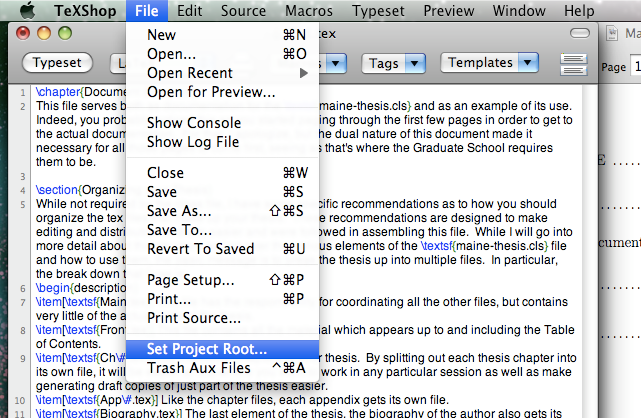
\includegraphics[height=2in]{Figures/ProjectRoot}
\caption[``Set Project Root...'' option in the File menu for TeXShop.]{``Set Project Root...'' option in the File menu for TeXShop.  This option is no longer a menu item in the most recent version of TeXShop but this figure is retained here as an example of figure usage.}
\label{rootmenu}
\end{figure}

\begin{figure}
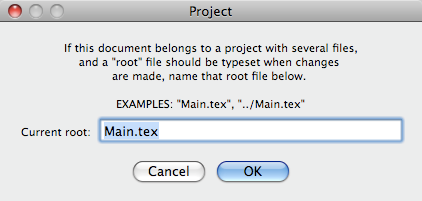
\includegraphics[height=2in]{Figures/Dialog}
\caption[``Set Project Root...'' dialog for TeXShop. ]{``Set Project Root...'' dialog for TeXShop.  This option is no longer a menu item in the most recent version of TeXShop but this figure is retained here as an example of figure usage.}
\label{rootdialog}
\end{figure}

If you're not using TeXShop or TeXWorks, then I suggest consulting the user manual or help files for your particular editor to figure out how to set the project root for a file.

\section{Organization of this document}
If you've read the Table of Contents, you've no doubt noticed that each of the chapters in this document deals with one of the files listed above.  In that chapter you'll find instructions for what has to be in that file.  For the most part these are requirements of either the Graduate School or the maine-thesis.cls itself.  Deviation from them may result in your document not typesetting correctly or in it not conforming to the Graduate School guidelines.  If you follow all these instructions perfectly and the Graduate School still rejects your thesis on the basis of some formatting error, please contact me (\email) with a full description of the problem that the Graduate School had with your thesis and I will make every effort to update the class file as quickly as possible.

\section{Reporting a Bug or Formatting Problem}
If you find a bug with this class file, please create a minimal working example which reproduces the bug and email it to \email\ along with a description of the bug and any possible fixes you have tried (and whether they worked or not).  For those not familiar with it, there are a couple of good descriptions on the web:
\begin{itemize}
\item{\url{http://www.tex.ac.uk/cgi-bin/texfaq2html?label=minxampl}}
\item{\url{http://www.minimalbeispiel.de/mini-en.html}}
\end{itemize}

If you find a formatting problem with this class file, please create a minimal working example which reproduces the problem and email it to \email\ along with a description of the formatting problem.  If the problem was pointed out to you by the Graduate School, please indicate who in the Graduate School pointed the problem so that I can consult with them directly if needed.  If available, a document which demonstrates what the desired formatting looks like should also be included.

I cannot guarantee any timeline on how quickly bugs or formatting problems will be dealt with, but I will make every effort to correct them as quickly as possible.

\endinput				% Chapter 1
% !TEX root =  Main.tex
\chapter{Main.tex}
Main.tex is responsible for 5 things:
\begin{enumerate}
\item{the loading of the class file and any packages you need to properly typeset your thesis,}
\item{the declaration of the principal variables in the thesis (author, title, advisor, etc.),}
\item{coordinating which files should be typeset at this particular time,}
\item{typesetting the title page of the thesis, and}
\item{placing and typesetting the references according to the style file you select.}
\end{enumerate}
We shall deal with each of these, though not necessarily in the order listed above.

\section{Class and Package Loading}\label{class}
Like any other \LaTeX\ project, a thesis set using maine-thesis.cls must start with a declaration of the document class:

\begin{verbatim}
\documentclass[options]{maine-thesis}
\end{verbatim}

\pagebreak[3]The options are as follows:
\begin{description}
\item[10pt]{This option sets the font size to 10pt.  This option is allowed by the graduate school for an official copy, but is not recommended (the smaller font size doesn't convert to microfilm as well as the default).}
\item[11pt]{This option sets the font size to 11pt.  This option is allowed by the graduate school for an official copy, but is not recommended (the smaller font size doesn't convert to microfilm as well as the default).}
\item[12pt]{This option sets the font size to 12pt.  This is the default option, and doesn't normally need to be issued.}
\item[apa]{This option changes the headings to follow the American Psychology Association style with one exception: italics are replaced by underlines (since italics in the headings is prohibited by the Graduate School).  These heading styles are unnumbered and thus cross references using \verb=\ref= will point to just the chapter.}
\item[chicago]{This option changes the headings to follow the Chicago style guidelines.  These heading styles are unnumbered and thus cross references using \verb=\ref= will point to just the chapter.}
\item[headings]{This option changes the headings to follow the example given in the Guidelines for unnumbered headings.  As they are unnumbered, cross references using \verb=\ref= will point to just the chapter.}
\item[idecimal]{This option changes the headings to follow the indented decimal example given in the Guidelines.}
\item[jdecimal]{This option is the default headings system (so you don't need to give it explicitly) and matches the left-justified decimal example given in the Guidelines.}
\end{description}

All of the above options are permitted in the official copy of your these.  There are also several options which are intended to help you create copies of your thesis which are intended for some other purpose.  They may not be used in the official copy of your thesis.  These options are as follows:

\begin{description}
\item[draft]{This option does a few things:
	\begin{itemize}
	\item{it marks the copy of the file as a draft by placing DRAFT in all four corners of each page (moving the page number to the bottom center if the top page style was selected),}
	\item{it marks any over full line with a black rectangle at the end,}
	\item{it allows \verb=\comment{...}= commands to show in the outside margin (right-hand normally, but if twoside is also given, then it's the left-hand margin on even pages),}
	\item{it places the current date in the top center of each page, and}
	\item{it sets the font size to 10pt to reduce the document page count and save paper.}
	\end{itemize}
Taken together, these changes make this option useful when you want to distribute copies of your thesis (or parts thereof) to someone for feedback prior to completing it.}
\item[twoside]{This option sets the margins to allow for binding of a two sided printing.  Thus odd number pages have a larger left-hand margin while even number pages have a larger right-hand margin.  Chapters (or chapter equivalent elements) will always begin on an odd page.  It also moves the page number for even pages to the upper left-hand corner for the top page style so that page numbers are always on the outer edge of the bound copy. 
Taken together, these changes make this option useful for producing extra copies of your thesis that you want bound for your advisor, your committee members, yourself, or other people.  It will reduce your paper usage nearly in half (more than that if you also use a smaller font).}
\item[unbound]{This option sets the margins to equal width, widening the text area in the process.  It is thus suitable for creating copies which will not be bound and thus don't need the extra wide margin to one side.  If issued with the twoside option, the margins and text width specified here will override those for two-sided printing, but the other aspects of two-sided printing remain in effect.}
\end{description}
If you issue more than one of the font size options, only the largest one will take effect.  However, the draft option will always change the font size to 10pt, regardless of any other options issued.  If you have the tex files for this documentation, you can see the effects of each of these options by editing the document class declaration in Main.tex and re-typsetting the document.

Once you have declared the document class, it's time to load packages.  There are far too many of these for me to possibly cover them all, but ones which have known issues are listed in Appendix \ref{package}.

\section{Variable Declarations}

Once you've initialized all the stuff you need to typeset your document, it's time to start adding content.  Since many elements of this content get used over and over again, the class file allows for you to declare them once and then places them in all the appropriate places.

\subsection{Describe Yourself}\label{self}
The first batch of these variables that you'll declare are the title of your thesis, your name, the degrees you already hold, the degree you're going for, the specialty in which this degree is, and when you are graduating.  These are declared with some fairly self explanatory commands:

\begin{verbatim}
\title{...}
\author{...}
\degreesheld{...}
\degree{...}
\program{...}
\submitdate{...}
\end{verbatim}

Note that you should use \verb=\\= to separate multiple degrees if you have more than one.  This will place them on separate lines (a Graduate School requirement).  Also, your submit date should be ``May,'' ``August,'' or ``December'' and the appropriate year.

\subsection{Describe Your Committee}\label{comm}
Next, you'll want to tell the class file about your committee.  To do this, you'll need each committee member's full name and title (i.e. Ph.D., faculty position, etc., as in ``John Smith, Ph.D., Associate Professor of Interesting Stuff'').  Each member is declared with a separate command (use only the ones you need):

\begin{verbatim}
\principaladvisor[...]{...}
\secondadvisor{...}

\firstreader{...}
\secondreader{...}
\thirdreader{...}
\fourthreader{...}
\fifthreader{...}
\end{verbatim}

Note that these commands are order sensitive as the class file uses the last one called to determine the number of committee members.  I.e. if you call \verb=\thirdreader{...}= after \verb=\fifthreader{...}= then the class file will think that you have 3 committee members beyond your advisor(s) rather than 5.

If this automatic numbering of your committee isn't working for some reason, then there are two commands which you can issue after the members list to override the behavior: \verb=\twoadvisors=, \verb=\oneadvisor= and \verb=\members{#}=.  The first is used to change the number of advisors to two, the second sets it to one (one advisor is the default for the class file).  The last tells the class file how many members your committee has (not including your advisor(s)).  If you find that you have to issue these commands, please send me a minimal working example that duplicates the problem you experienced so that I can fix it.

In a couple of locations, the thesis requires the ``short'' name for your advisor.  In this case, the advisor's title should simply be ``Dr.'' (or whatever is appropriate) and should precede their name (as in ``Dr.~John Smith'').  This short name can be defined in two ways.  If you have just one advisor, then you can make use of the first (optional) argument of \verb=\prinicpaladvisor= (the one appearing between the square brackets):

\begin{verbatim}
\principaladvisor[Dr.~John Smith]{John Smith, Ph.D., Associate Professor of Interesting Stuff}
\end{verbatim}

If you have two advisors, then you should leave out the first argument for \verb=\prinicpaladvisor= and use the command \verb=\prinicpalshort= instead.  For this command both names should appear as the argument to the command with their short titles separate:

\begin{verbatim}
\principaladvisor{John Smith, Ph.D., Associate Professor of Interesting Stuff}
\secondadvisor{Jane Doe, Ph.D., Professor of More Interesting Stuff}
\principalshort{Dr.~John Smith and Dr.~Jane Doe}
\end{verbatim}

\subsection{Number of Appendices}
If you have more than one appendix, then you have to tell the class file this with the command \verb=\multipleappendicestrue=.  This is because the Graduate School requires different formatting for a document with a single appendix as opposed to one with multiple appendices (in particular as relating to lettering them and how they appear in the table of contents).  By default, the class file assumes one appendix and will format it accordingly.  If you have more than one, then this command will tell the class file to change to the multiple appendices format.  If you don't have any appendices, then it shouldn't matter if you issue this command or not.

\subsection{Document Type}
By default, the class file will refer to your document as a dissertation.  If your degree program refers to it as a thesis or project, then you'll want to tell the class file that.  The command \verb=\thesis= will change all occurrences of ``dissertation'' to ``thesis'' and \verb=\project= will change them to ``project.''

\section{Title page}

Now that all the variables are declared, it's time to start the document itself.  This consists of three commands:

\begin{verbatim}
\begin{document}
\preliminary
\titlepage
\end{verbatim}

The first is the usual command that tells \LaTeX\ where the document starts.  The second tells the class file that what comes next is the front matter of the thesis.  This means that pages should be numbered with lowercase roman numerals.  The last command creates the title page.  Putting it here ensures that every copy of your thesis that you create will include a copy of the title page, making it easier to identify the document (especially important when you're handing out bits and pieces).

After the title page, it's time to include the rest of the preliminary material, but I don't suggest putting all of that in Main.tex.  Instead, all of that should be put in Front.tex, a process which gets us to our next job for Main.tex: coordinating which files are to be processed at this time.

\section{File Coordination}
Chances are pretty good that your final thesis will be close to, if not well over, 100 pages.  If all of that material were in a single file, finding where it is you want to edit something can be difficult.  To make this easier, \LaTeX\ allows you to split the document up into multiple files and then use the \verb=\include{...}= statement to tell the main file to add the contents of another file at this point.  We're going to make use of that here.  First off, we'll place all the front matter (copyright page, dissertation acceptance statement, library rights statement, abstract(s), preface, dedication, acknowledgements, and table of contents):

\begin{verbatim}
% !TEX root =  Main.tex
%\preparetocs
\dissacceptance
\copyrightpage[<Copyright holder appears here, see Section \ref{copy} for details>]{<Copyright year appears here>}
\libraryrights

\begin{abstract}
The abstract for you thesis will appear on this page.  It should be limited to 350 words for a Ph.D thesis or 500 words for a Master's thesis.
\end{abstract}

\begin{layabstract}{Lay abstract keywords appear here}
The Grad School now requires a lay abstract of up to 350 words for all theses, but also requires that the lay abstract be submitted electronically to Cyrstal Burgess (email: \verb=crystal.burgess@maine.edu=).  Whether you include it in the bound version of your thesis is your choice.

If you do want to include the lay abstract in the bound version of your thesis then it will appear here.
\end{layabstract}

\begin{preface}
\section{Preface from the 2003 version}

 This class file is written for use with the \LaTeXe\ document preparation system for theses
 conforming to the guidelines of the Graduate School at the University of Maine.  
 Ideas for this class were found in  
 the class files \verb=gt-thesis.cls=\footnote{available at
 http://www.ctan.org} and \verb=rpithesis.cls=.\footnote{can be currently found at
  http://www.rpi.edu/computing/software/latex/thesis-info.html}  This class
 file is relatively compact, without too many options for the user.  A majority of the
 credit for this class should go to the original writers of those two classes.  

 \paragraph{What This Class File Can Do---}
 \verb=maine-thesis.cls= can format a masters or doctoral thesis according to the guidelines set
 forth by the Graduate School of the University of Maine.  It produces a double spaced, one sided
 document with the correct margins for final publication. 
 It will properly format a titlepage, 
 optional copyright page, abstract, optional dedication, acknowledgements and preface sections,
 a table of contents, lists of tables and figures, main matter, and end matter.  The Graduate
 School is relatively lenient in some formatting issues and strict in others.  Where there is
 leniency, decisions were made that I thought looked best.  Changes can be made to the class file
 to make it look more to your liking, but in its current version, this class file
 will produce a thesis that is acceptable to the Graduate School.
 \paragraph{A Final Note---}
 A word of warning:  {\bfseries THE GUIDELINES OF THE GRADUATE SCHOOL CAN AND DO CHANGE.}	
 This class was written using the most recent set of guidelines [...]\footnote{Date of the guidelines used by the original package author has been removed to avoid confusion.}.  
 They do change every so often so be sure that you have a copy of the most recent set of
 guidelines.  Most changes that are made will probably be small and cosmetic but there is no guarantee that
 something major will not arise.  
 
 \begin{flushright}
 Jim Kenneally
 \end{flushright}
 
\section{Preface to version 1.5}
As Jim predicted, the guidelines of the graduate school have changed a bit over the years since he originally designed this class file.  Over those intervening years every successive person who has used the class file has been required by the Graduate School to make some changes: some in response to things which Jim didn't get quite right, most to things which they had changed or become stricter on.  In most cases those changes accumulated in various versions of the file and were handed on to the next person interested in using the class file.  In some cases, however, a student would leave before they handed the class file on to anyone and as a result any changes they made would be lost and have to be reproduced.

I've made the effort to acquire all versions of the class file that I can and to consolidate the changes they contain into a single project.  I've also requested feedback from the Graduate School to make sure that this package conforms to their current standards.  This is the result.  I hope you find it useful and easy to use.

If the Graduate School requires you to change some aspect of your thesis formatting which you believe should be taken care of by this class file, please email me (\email) with a detailed description of the problem and a simple sample document that reproduces it (I don't want your whole thesis, just the part that's not right).  While I cannot guarantee that I will get to it right away, I will look at the problem just as soon as I have time and will endeavor to fix it.  If you can't afford to wait for me to fix the problem and find a fix that works, please email me that fix as well, as it's much easier for me to incorporate a fix than it is to diagnose and fix a problem.

As of April 2016, this thesis class is now hosted on GitHub (\url{https://github.com/rpspringuel/maine-thesis}).  If you have a GitHub account (they are free), you can submit Issues (bug reports) and Pull Requests (suggested changes) there.

\begin{flushright}
R. Padraic Springuel\\
Most recent version of Graduate School guidelines used: June 2015\\
Documentation last edited on \today
\end{flushright}

\end{preface}

\begin{dedication}
Dedications are optional, but if you have one it will appear here.
\end{dedication}

\begin{acknowledgements}
While acknowledgements are technically optional, they are also the perfect place to make note of funding sources, collaborators, and other people whose work made your thesis possible.  This is also the place to mention an External Reader (i.e. some one from outside the University who read and commented on your thesis) if you have one.  Acknowledgements appear here.
\end{acknowledgements}

\tableofcontents
\listoftables
\listoffigures

\begin{listof}{Whatever}
If you have some an consistent set of theorems, symbols, abbreviations, or definitions, then you must include a page which lists them just as you list the tables and figures in your thesis.
\end{listof}

\mainmatter{bottom}

\endinput
\end{verbatim}

Next comes the main body of the thesis, which is just a bunch of \verb=\include{...}= statements: one for each chapter:

\begin{verbatim}
% !TEX root =  Main.tex
\chapter{Introduction}
This file serves both as documentation for the maine-thesis.cls and as an example of its use.  Indeed, you probably noticed this as you started paging through the first few pages in order to get to the actual documentation.  For that, I apologize, but the dual nature of this document made it necessary for all those pages to come first, seeing as that's where the Graduate School requires them to be.

This document is not intended to be an introduction on how to use \LaTeX. In fact, I will assume that you are familiar with basic \LaTeX\ commands and have typeset documents in \LaTeX\ before throughout this document.  If you haven't, then I highly suggest finding a reference book or tutorial that will teach you the basics of \LaTeX\ and read through that first.  There are several options available both in print and online (e.g. \cite{Kopka:2004,Mittelbach:2004,Flynn:2005}).  Which one you use is largely a matter of preference.

\section{Installation}
To install this class file you need to place it in \verb=~=/texmf/tex/latex/ where the ``\verb=~='' represents the location of your local texmf directory.\footnote{The final path should not have .../texmf/texmf/... in it, just .../texmf/...}  Since this changes from system to system, I can't be more specific than that, so check the documentation for your system.

\section{Organizing your Thesis}
While not required by the class file, I have some specific recommendations as to how you should organize the tex files that make up your thesis.  These recommendations are designed to make editing and distribution of drafts easier and were followed in assembling this document.  While I will go into more detail about this structure as I go over the various elements of the maine-thesis.cls file and how to use them, the basic message is to break the thesis up into multiple files.  In particular, the break down that I use is:
\begin{description}
\item[Main.tex] This file has the responsibility for coordinating all the other files, but contains very little of the actual body of the thesis.
\item[Front.tex] This file contains all the material which appears up to and including the Table of Contents.
\item[Ch\#.tex] The individual chapters of your thesis.  By splitting out each thesis chapter into its own file, it will be easier to find where you want to work in any particular session as well as make generating draft copies of just part of the thesis easier.
\item[App\#.tex] Like the chapter files, each appendix gets its own file.
\item[Biography.tex] The last element of the thesis, the biography of the author also gets its own file to avoid adding clutter to Main.tex.
\item[Figures] Since most of the figures you use in your thesis are likely to be separate image files which \LaTeX\ will need access to when it typesets your thesis, I advise making a subfolder for your project where you can place these images.  It'll make them easier to find later when you need to change them and keep the project root folder from getting too cluttered.
\end{description}

All of these files should be located in a single folder specifically created for this purpose.  Since \LaTeX\ creates several files when typesetting documents, this will keep all those files in one place and keep them from crowding up your usual documents folders.

In this documentation, I will be assuming that the above organization structure is in use.  If you're using something else, you'll have to modify the instructions provided here accordingly.

If you are using these guidelines, however, it is highly useful if you set Main.tex as the root project file for all other files in your \LaTeX\ editor.  You'll get fewer errors this way as you'll be able to order your editor to typeset the project without switching to Main.tex first, regardless of which file you're currently working on.

While I can't provide you with exact instructions for this process for every possible editor, in TeXShop or TeXWorks, simply add the line ``\verb|% !TEX root =  Main.tex|'' to top of each chapter file.

\begin{figure}
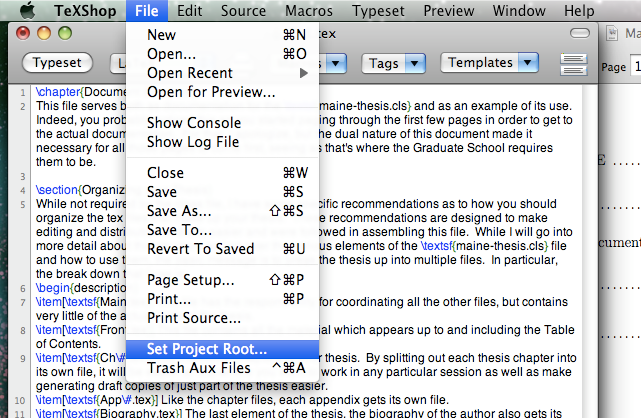
\includegraphics[height=2in]{Figures/ProjectRoot}
\caption[``Set Project Root...'' option in the File menu for TeXShop.]{``Set Project Root...'' option in the File menu for TeXShop.  This option is no longer a menu item in the most recent version of TeXShop but this figure is retained here as an example of figure usage.}
\label{rootmenu}
\end{figure}

\begin{figure}
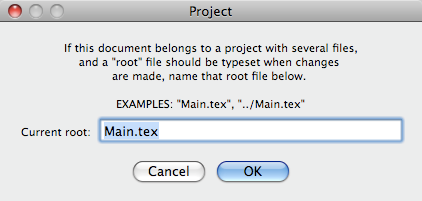
\includegraphics[height=2in]{Figures/Dialog}
\caption[``Set Project Root...'' dialog for TeXShop. ]{``Set Project Root...'' dialog for TeXShop.  This option is no longer a menu item in the most recent version of TeXShop but this figure is retained here as an example of figure usage.}
\label{rootdialog}
\end{figure}

If you're not using TeXShop or TeXWorks, then I suggest consulting the user manual or help files for your particular editor to figure out how to set the project root for a file.

\section{Organization of this document}
If you've read the Table of Contents, you've no doubt noticed that each of the chapters in this document deals with one of the files listed above.  In that chapter you'll find instructions for what has to be in that file.  For the most part these are requirements of either the Graduate School or the maine-thesis.cls itself.  Deviation from them may result in your document not typesetting correctly or in it not conforming to the Graduate School guidelines.  If you follow all these instructions perfectly and the Graduate School still rejects your thesis on the basis of some formatting error, please contact me (\email) with a full description of the problem that the Graduate School had with your thesis and I will make every effort to update the class file as quickly as possible.

\section{Reporting a Bug or Formatting Problem}
If you find a bug with this class file, please create a minimal working example which reproduces the bug and email it to \email\ along with a description of the bug and any possible fixes you have tried (and whether they worked or not).  For those not familiar with it, there are a couple of good descriptions on the web:
\begin{itemize}
\item{\url{http://www.tex.ac.uk/cgi-bin/texfaq2html?label=minxampl}}
\item{\url{http://www.minimalbeispiel.de/mini-en.html}}
\end{itemize}

If you find a formatting problem with this class file, please create a minimal working example which reproduces the problem and email it to \email\ along with a description of the formatting problem.  If the problem was pointed out to you by the Graduate School, please indicate who in the Graduate School pointed the problem so that I can consult with them directly if needed.  If available, a document which demonstrates what the desired formatting looks like should also be included.

I cannot guarantee any timeline on how quickly bugs or formatting problems will be dealt with, but I will make every effort to correct them as quickly as possible.

\endinput
% !TEX root =  Main.tex
\chapter{Main.tex}
Main.tex is responsible for 5 things:
\begin{enumerate}
\item{the loading of the class file and any packages you need to properly typeset your thesis,}
\item{the declaration of the principal variables in the thesis (author, title, advisor, etc.),}
\item{coordinating which files should be typeset at this particular time,}
\item{typesetting the title page of the thesis, and}
\item{placing and typesetting the references according to the style file you select.}
\end{enumerate}
We shall deal with each of these, though not necessarily in the order listed above.

\section{Class and Package Loading}\label{class}
Like any other \LaTeX\ project, a thesis set using maine-thesis.cls must start with a declaration of the document class:

\begin{verbatim}
\documentclass[options]{maine-thesis}
\end{verbatim}

\pagebreak[3]The options are as follows:
\begin{description}
\item[10pt]{This option sets the font size to 10pt.  This option is allowed by the graduate school for an official copy, but is not recommended (the smaller font size doesn't convert to microfilm as well as the default).}
\item[11pt]{This option sets the font size to 11pt.  This option is allowed by the graduate school for an official copy, but is not recommended (the smaller font size doesn't convert to microfilm as well as the default).}
\item[12pt]{This option sets the font size to 12pt.  This is the default option, and doesn't normally need to be issued.}
\item[apa]{This option changes the headings to follow the American Psychology Association style with one exception: italics are replaced by underlines (since italics in the headings is prohibited by the Graduate School).  These heading styles are unnumbered and thus cross references using \verb=\ref= will point to just the chapter.}
\item[chicago]{This option changes the headings to follow the Chicago style guidelines.  These heading styles are unnumbered and thus cross references using \verb=\ref= will point to just the chapter.}
\item[headings]{This option changes the headings to follow the example given in the Guidelines for unnumbered headings.  As they are unnumbered, cross references using \verb=\ref= will point to just the chapter.}
\item[idecimal]{This option changes the headings to follow the indented decimal example given in the Guidelines.}
\item[jdecimal]{This option is the default headings system (so you don't need to give it explicitly) and matches the left-justified decimal example given in the Guidelines.}
\end{description}

All of the above options are permitted in the official copy of your these.  There are also several options which are intended to help you create copies of your thesis which are intended for some other purpose.  They may not be used in the official copy of your thesis.  These options are as follows:

\begin{description}
\item[draft]{This option does a few things:
	\begin{itemize}
	\item{it marks the copy of the file as a draft by placing DRAFT in all four corners of each page (moving the page number to the bottom center if the top page style was selected),}
	\item{it marks any over full line with a black rectangle at the end,}
	\item{it allows \verb=\comment{...}= commands to show in the outside margin (right-hand normally, but if twoside is also given, then it's the left-hand margin on even pages),}
	\item{it places the current date in the top center of each page, and}
	\item{it sets the font size to 10pt to reduce the document page count and save paper.}
	\end{itemize}
Taken together, these changes make this option useful when you want to distribute copies of your thesis (or parts thereof) to someone for feedback prior to completing it.}
\item[twoside]{This option sets the margins to allow for binding of a two sided printing.  Thus odd number pages have a larger left-hand margin while even number pages have a larger right-hand margin.  Chapters (or chapter equivalent elements) will always begin on an odd page.  It also moves the page number for even pages to the upper left-hand corner for the top page style so that page numbers are always on the outer edge of the bound copy. 
Taken together, these changes make this option useful for producing extra copies of your thesis that you want bound for your advisor, your committee members, yourself, or other people.  It will reduce your paper usage nearly in half (more than that if you also use a smaller font).}
\item[unbound]{This option sets the margins to equal width, widening the text area in the process.  It is thus suitable for creating copies which will not be bound and thus don't need the extra wide margin to one side.  If issued with the twoside option, the margins and text width specified here will override those for two-sided printing, but the other aspects of two-sided printing remain in effect.}
\end{description}
If you issue more than one of the font size options, only the largest one will take effect.  However, the draft option will always change the font size to 10pt, regardless of any other options issued.  If you have the tex files for this documentation, you can see the effects of each of these options by editing the document class declaration in Main.tex and re-typsetting the document.

Once you have declared the document class, it's time to load packages.  There are far too many of these for me to possibly cover them all, but ones which have known issues are listed in Appendix \ref{package}.

\section{Variable Declarations}

Once you've initialized all the stuff you need to typeset your document, it's time to start adding content.  Since many elements of this content get used over and over again, the class file allows for you to declare them once and then places them in all the appropriate places.

\subsection{Describe Yourself}\label{self}
The first batch of these variables that you'll declare are the title of your thesis, your name, the degrees you already hold, the degree you're going for, the specialty in which this degree is, and when you are graduating.  These are declared with some fairly self explanatory commands:

\begin{verbatim}
\title{...}
\author{...}
\degreesheld{...}
\degree{...}
\program{...}
\submitdate{...}
\end{verbatim}

Note that you should use \verb=\\= to separate multiple degrees if you have more than one.  This will place them on separate lines (a Graduate School requirement).  Also, your submit date should be ``May,'' ``August,'' or ``December'' and the appropriate year.

\subsection{Describe Your Committee}\label{comm}
Next, you'll want to tell the class file about your committee.  To do this, you'll need each committee member's full name and title (i.e. Ph.D., faculty position, etc., as in ``John Smith, Ph.D., Associate Professor of Interesting Stuff'').  Each member is declared with a separate command (use only the ones you need):

\begin{verbatim}
\principaladvisor[...]{...}
\secondadvisor{...}

\firstreader{...}
\secondreader{...}
\thirdreader{...}
\fourthreader{...}
\fifthreader{...}
\end{verbatim}

Note that these commands are order sensitive as the class file uses the last one called to determine the number of committee members.  I.e. if you call \verb=\thirdreader{...}= after \verb=\fifthreader{...}= then the class file will think that you have 3 committee members beyond your advisor(s) rather than 5.

If this automatic numbering of your committee isn't working for some reason, then there are two commands which you can issue after the members list to override the behavior: \verb=\twoadvisors=, \verb=\oneadvisor= and \verb=\members{#}=.  The first is used to change the number of advisors to two, the second sets it to one (one advisor is the default for the class file).  The last tells the class file how many members your committee has (not including your advisor(s)).  If you find that you have to issue these commands, please send me a minimal working example that duplicates the problem you experienced so that I can fix it.

In a couple of locations, the thesis requires the ``short'' name for your advisor.  In this case, the advisor's title should simply be ``Dr.'' (or whatever is appropriate) and should precede their name (as in ``Dr.~John Smith'').  This short name can be defined in two ways.  If you have just one advisor, then you can make use of the first (optional) argument of \verb=\prinicpaladvisor= (the one appearing between the square brackets):

\begin{verbatim}
\principaladvisor[Dr.~John Smith]{John Smith, Ph.D., Associate Professor of Interesting Stuff}
\end{verbatim}

If you have two advisors, then you should leave out the first argument for \verb=\prinicpaladvisor= and use the command \verb=\prinicpalshort= instead.  For this command both names should appear as the argument to the command with their short titles separate:

\begin{verbatim}
\principaladvisor{John Smith, Ph.D., Associate Professor of Interesting Stuff}
\secondadvisor{Jane Doe, Ph.D., Professor of More Interesting Stuff}
\principalshort{Dr.~John Smith and Dr.~Jane Doe}
\end{verbatim}

\subsection{Number of Appendices}
If you have more than one appendix, then you have to tell the class file this with the command \verb=\multipleappendicestrue=.  This is because the Graduate School requires different formatting for a document with a single appendix as opposed to one with multiple appendices (in particular as relating to lettering them and how they appear in the table of contents).  By default, the class file assumes one appendix and will format it accordingly.  If you have more than one, then this command will tell the class file to change to the multiple appendices format.  If you don't have any appendices, then it shouldn't matter if you issue this command or not.

\subsection{Document Type}
By default, the class file will refer to your document as a dissertation.  If your degree program refers to it as a thesis or project, then you'll want to tell the class file that.  The command \verb=\thesis= will change all occurrences of ``dissertation'' to ``thesis'' and \verb=\project= will change them to ``project.''

\section{Title page}

Now that all the variables are declared, it's time to start the document itself.  This consists of three commands:

\begin{verbatim}
\begin{document}
\preliminary
\titlepage
\end{verbatim}

The first is the usual command that tells \LaTeX\ where the document starts.  The second tells the class file that what comes next is the front matter of the thesis.  This means that pages should be numbered with lowercase roman numerals.  The last command creates the title page.  Putting it here ensures that every copy of your thesis that you create will include a copy of the title page, making it easier to identify the document (especially important when you're handing out bits and pieces).

After the title page, it's time to include the rest of the preliminary material, but I don't suggest putting all of that in Main.tex.  Instead, all of that should be put in Front.tex, a process which gets us to our next job for Main.tex: coordinating which files are to be processed at this time.

\section{File Coordination}
Chances are pretty good that your final thesis will be close to, if not well over, 100 pages.  If all of that material were in a single file, finding where it is you want to edit something can be difficult.  To make this easier, \LaTeX\ allows you to split the document up into multiple files and then use the \verb=\include{...}= statement to tell the main file to add the contents of another file at this point.  We're going to make use of that here.  First off, we'll place all the front matter (copyright page, dissertation acceptance statement, library rights statement, abstract(s), preface, dedication, acknowledgements, and table of contents):

\begin{verbatim}
% !TEX root =  Main.tex
%\preparetocs
\dissacceptance
\copyrightpage[<Copyright holder appears here, see Section \ref{copy} for details>]{<Copyright year appears here>}
\libraryrights

\begin{abstract}
The abstract for you thesis will appear on this page.  It should be limited to 350 words for a Ph.D thesis or 500 words for a Master's thesis.
\end{abstract}

\begin{layabstract}{Lay abstract keywords appear here}
The Grad School now requires a lay abstract of up to 350 words for all theses, but also requires that the lay abstract be submitted electronically to Cyrstal Burgess (email: \verb=crystal.burgess@maine.edu=).  Whether you include it in the bound version of your thesis is your choice.

If you do want to include the lay abstract in the bound version of your thesis then it will appear here.
\end{layabstract}

\begin{preface}
\section{Preface from the 2003 version}

 This class file is written for use with the \LaTeXe\ document preparation system for theses
 conforming to the guidelines of the Graduate School at the University of Maine.  
 Ideas for this class were found in  
 the class files \verb=gt-thesis.cls=\footnote{available at
 http://www.ctan.org} and \verb=rpithesis.cls=.\footnote{can be currently found at
  http://www.rpi.edu/computing/software/latex/thesis-info.html}  This class
 file is relatively compact, without too many options for the user.  A majority of the
 credit for this class should go to the original writers of those two classes.  

 \paragraph{What This Class File Can Do---}
 \verb=maine-thesis.cls= can format a masters or doctoral thesis according to the guidelines set
 forth by the Graduate School of the University of Maine.  It produces a double spaced, one sided
 document with the correct margins for final publication. 
 It will properly format a titlepage, 
 optional copyright page, abstract, optional dedication, acknowledgements and preface sections,
 a table of contents, lists of tables and figures, main matter, and end matter.  The Graduate
 School is relatively lenient in some formatting issues and strict in others.  Where there is
 leniency, decisions were made that I thought looked best.  Changes can be made to the class file
 to make it look more to your liking, but in its current version, this class file
 will produce a thesis that is acceptable to the Graduate School.
 \paragraph{A Final Note---}
 A word of warning:  {\bfseries THE GUIDELINES OF THE GRADUATE SCHOOL CAN AND DO CHANGE.}	
 This class was written using the most recent set of guidelines [...]\footnote{Date of the guidelines used by the original package author has been removed to avoid confusion.}.  
 They do change every so often so be sure that you have a copy of the most recent set of
 guidelines.  Most changes that are made will probably be small and cosmetic but there is no guarantee that
 something major will not arise.  
 
 \begin{flushright}
 Jim Kenneally
 \end{flushright}
 
\section{Preface to version 1.5}
As Jim predicted, the guidelines of the graduate school have changed a bit over the years since he originally designed this class file.  Over those intervening years every successive person who has used the class file has been required by the Graduate School to make some changes: some in response to things which Jim didn't get quite right, most to things which they had changed or become stricter on.  In most cases those changes accumulated in various versions of the file and were handed on to the next person interested in using the class file.  In some cases, however, a student would leave before they handed the class file on to anyone and as a result any changes they made would be lost and have to be reproduced.

I've made the effort to acquire all versions of the class file that I can and to consolidate the changes they contain into a single project.  I've also requested feedback from the Graduate School to make sure that this package conforms to their current standards.  This is the result.  I hope you find it useful and easy to use.

If the Graduate School requires you to change some aspect of your thesis formatting which you believe should be taken care of by this class file, please email me (\email) with a detailed description of the problem and a simple sample document that reproduces it (I don't want your whole thesis, just the part that's not right).  While I cannot guarantee that I will get to it right away, I will look at the problem just as soon as I have time and will endeavor to fix it.  If you can't afford to wait for me to fix the problem and find a fix that works, please email me that fix as well, as it's much easier for me to incorporate a fix than it is to diagnose and fix a problem.

As of April 2016, this thesis class is now hosted on GitHub (\url{https://github.com/rpspringuel/maine-thesis}).  If you have a GitHub account (they are free), you can submit Issues (bug reports) and Pull Requests (suggested changes) there.

\begin{flushright}
R. Padraic Springuel\\
Most recent version of Graduate School guidelines used: June 2015\\
Documentation last edited on \today
\end{flushright}

\end{preface}

\begin{dedication}
Dedications are optional, but if you have one it will appear here.
\end{dedication}

\begin{acknowledgements}
While acknowledgements are technically optional, they are also the perfect place to make note of funding sources, collaborators, and other people whose work made your thesis possible.  This is also the place to mention an External Reader (i.e. some one from outside the University who read and commented on your thesis) if you have one.  Acknowledgements appear here.
\end{acknowledgements}

\tableofcontents
\listoftables
\listoffigures

\begin{listof}{Whatever}
If you have some an consistent set of theorems, symbols, abbreviations, or definitions, then you must include a page which lists them just as you list the tables and figures in your thesis.
\end{listof}

\mainmatter{bottom}

\endinput
\end{verbatim}

Next comes the main body of the thesis, which is just a bunch of \verb=\include{...}= statements: one for each chapter:

\begin{verbatim}
% !TEX root =  Main.tex
\chapter{Introduction}
This file serves both as documentation for the maine-thesis.cls and as an example of its use.  Indeed, you probably noticed this as you started paging through the first few pages in order to get to the actual documentation.  For that, I apologize, but the dual nature of this document made it necessary for all those pages to come first, seeing as that's where the Graduate School requires them to be.

This document is not intended to be an introduction on how to use \LaTeX. In fact, I will assume that you are familiar with basic \LaTeX\ commands and have typeset documents in \LaTeX\ before throughout this document.  If you haven't, then I highly suggest finding a reference book or tutorial that will teach you the basics of \LaTeX\ and read through that first.  There are several options available both in print and online (e.g. \cite{Kopka:2004,Mittelbach:2004,Flynn:2005}).  Which one you use is largely a matter of preference.

\section{Installation}
To install this class file you need to place it in \verb=~=/texmf/tex/latex/ where the ``\verb=~='' represents the location of your local texmf directory.\footnote{The final path should not have .../texmf/texmf/... in it, just .../texmf/...}  Since this changes from system to system, I can't be more specific than that, so check the documentation for your system.

\section{Organizing your Thesis}
While not required by the class file, I have some specific recommendations as to how you should organize the tex files that make up your thesis.  These recommendations are designed to make editing and distribution of drafts easier and were followed in assembling this document.  While I will go into more detail about this structure as I go over the various elements of the maine-thesis.cls file and how to use them, the basic message is to break the thesis up into multiple files.  In particular, the break down that I use is:
\begin{description}
\item[Main.tex] This file has the responsibility for coordinating all the other files, but contains very little of the actual body of the thesis.
\item[Front.tex] This file contains all the material which appears up to and including the Table of Contents.
\item[Ch\#.tex] The individual chapters of your thesis.  By splitting out each thesis chapter into its own file, it will be easier to find where you want to work in any particular session as well as make generating draft copies of just part of the thesis easier.
\item[App\#.tex] Like the chapter files, each appendix gets its own file.
\item[Biography.tex] The last element of the thesis, the biography of the author also gets its own file to avoid adding clutter to Main.tex.
\item[Figures] Since most of the figures you use in your thesis are likely to be separate image files which \LaTeX\ will need access to when it typesets your thesis, I advise making a subfolder for your project where you can place these images.  It'll make them easier to find later when you need to change them and keep the project root folder from getting too cluttered.
\end{description}

All of these files should be located in a single folder specifically created for this purpose.  Since \LaTeX\ creates several files when typesetting documents, this will keep all those files in one place and keep them from crowding up your usual documents folders.

In this documentation, I will be assuming that the above organization structure is in use.  If you're using something else, you'll have to modify the instructions provided here accordingly.

If you are using these guidelines, however, it is highly useful if you set Main.tex as the root project file for all other files in your \LaTeX\ editor.  You'll get fewer errors this way as you'll be able to order your editor to typeset the project without switching to Main.tex first, regardless of which file you're currently working on.

While I can't provide you with exact instructions for this process for every possible editor, in TeXShop or TeXWorks, simply add the line ``\verb|% !TEX root =  Main.tex|'' to top of each chapter file.

\begin{figure}
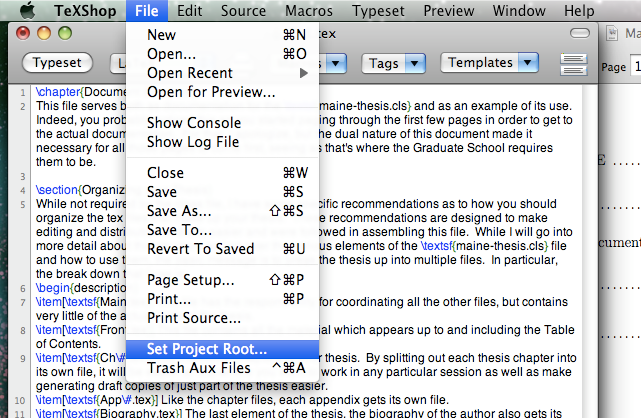
\includegraphics[height=2in]{Figures/ProjectRoot}
\caption[``Set Project Root...'' option in the File menu for TeXShop.]{``Set Project Root...'' option in the File menu for TeXShop.  This option is no longer a menu item in the most recent version of TeXShop but this figure is retained here as an example of figure usage.}
\label{rootmenu}
\end{figure}

\begin{figure}
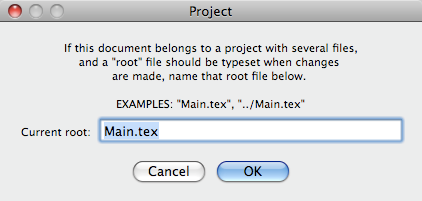
\includegraphics[height=2in]{Figures/Dialog}
\caption[``Set Project Root...'' dialog for TeXShop. ]{``Set Project Root...'' dialog for TeXShop.  This option is no longer a menu item in the most recent version of TeXShop but this figure is retained here as an example of figure usage.}
\label{rootdialog}
\end{figure}

If you're not using TeXShop or TeXWorks, then I suggest consulting the user manual or help files for your particular editor to figure out how to set the project root for a file.

\section{Organization of this document}
If you've read the Table of Contents, you've no doubt noticed that each of the chapters in this document deals with one of the files listed above.  In that chapter you'll find instructions for what has to be in that file.  For the most part these are requirements of either the Graduate School or the maine-thesis.cls itself.  Deviation from them may result in your document not typesetting correctly or in it not conforming to the Graduate School guidelines.  If you follow all these instructions perfectly and the Graduate School still rejects your thesis on the basis of some formatting error, please contact me (\email) with a full description of the problem that the Graduate School had with your thesis and I will make every effort to update the class file as quickly as possible.

\section{Reporting a Bug or Formatting Problem}
If you find a bug with this class file, please create a minimal working example which reproduces the bug and email it to \email\ along with a description of the bug and any possible fixes you have tried (and whether they worked or not).  For those not familiar with it, there are a couple of good descriptions on the web:
\begin{itemize}
\item{\url{http://www.tex.ac.uk/cgi-bin/texfaq2html?label=minxampl}}
\item{\url{http://www.minimalbeispiel.de/mini-en.html}}
\end{itemize}

If you find a formatting problem with this class file, please create a minimal working example which reproduces the problem and email it to \email\ along with a description of the formatting problem.  If the problem was pointed out to you by the Graduate School, please indicate who in the Graduate School pointed the problem so that I can consult with them directly if needed.  If available, a document which demonstrates what the desired formatting looks like should also be included.

I cannot guarantee any timeline on how quickly bugs or formatting problems will be dealt with, but I will make every effort to correct them as quickly as possible.

\endinput
% !TEX root =  Main.tex
\chapter{Main.tex}
Main.tex is responsible for 5 things:
\begin{enumerate}
\item{the loading of the class file and any packages you need to properly typeset your thesis,}
\item{the declaration of the principal variables in the thesis (author, title, advisor, etc.),}
\item{coordinating which files should be typeset at this particular time,}
\item{typesetting the title page of the thesis, and}
\item{placing and typesetting the references according to the style file you select.}
\end{enumerate}
We shall deal with each of these, though not necessarily in the order listed above.

\section{Class and Package Loading}\label{class}
Like any other \LaTeX\ project, a thesis set using maine-thesis.cls must start with a declaration of the document class:

\begin{verbatim}
\documentclass[options]{maine-thesis}
\end{verbatim}

\pagebreak[3]The options are as follows:
\begin{description}
\item[10pt]{This option sets the font size to 10pt.  This option is allowed by the graduate school for an official copy, but is not recommended (the smaller font size doesn't convert to microfilm as well as the default).}
\item[11pt]{This option sets the font size to 11pt.  This option is allowed by the graduate school for an official copy, but is not recommended (the smaller font size doesn't convert to microfilm as well as the default).}
\item[12pt]{This option sets the font size to 12pt.  This is the default option, and doesn't normally need to be issued.}
\item[apa]{This option changes the headings to follow the American Psychology Association style with one exception: italics are replaced by underlines (since italics in the headings is prohibited by the Graduate School).  These heading styles are unnumbered and thus cross references using \verb=\ref= will point to just the chapter.}
\item[chicago]{This option changes the headings to follow the Chicago style guidelines.  These heading styles are unnumbered and thus cross references using \verb=\ref= will point to just the chapter.}
\item[headings]{This option changes the headings to follow the example given in the Guidelines for unnumbered headings.  As they are unnumbered, cross references using \verb=\ref= will point to just the chapter.}
\item[idecimal]{This option changes the headings to follow the indented decimal example given in the Guidelines.}
\item[jdecimal]{This option is the default headings system (so you don't need to give it explicitly) and matches the left-justified decimal example given in the Guidelines.}
\end{description}

All of the above options are permitted in the official copy of your these.  There are also several options which are intended to help you create copies of your thesis which are intended for some other purpose.  They may not be used in the official copy of your thesis.  These options are as follows:

\begin{description}
\item[draft]{This option does a few things:
	\begin{itemize}
	\item{it marks the copy of the file as a draft by placing DRAFT in all four corners of each page (moving the page number to the bottom center if the top page style was selected),}
	\item{it marks any over full line with a black rectangle at the end,}
	\item{it allows \verb=\comment{...}= commands to show in the outside margin (right-hand normally, but if twoside is also given, then it's the left-hand margin on even pages),}
	\item{it places the current date in the top center of each page, and}
	\item{it sets the font size to 10pt to reduce the document page count and save paper.}
	\end{itemize}
Taken together, these changes make this option useful when you want to distribute copies of your thesis (or parts thereof) to someone for feedback prior to completing it.}
\item[twoside]{This option sets the margins to allow for binding of a two sided printing.  Thus odd number pages have a larger left-hand margin while even number pages have a larger right-hand margin.  Chapters (or chapter equivalent elements) will always begin on an odd page.  It also moves the page number for even pages to the upper left-hand corner for the top page style so that page numbers are always on the outer edge of the bound copy. 
Taken together, these changes make this option useful for producing extra copies of your thesis that you want bound for your advisor, your committee members, yourself, or other people.  It will reduce your paper usage nearly in half (more than that if you also use a smaller font).}
\item[unbound]{This option sets the margins to equal width, widening the text area in the process.  It is thus suitable for creating copies which will not be bound and thus don't need the extra wide margin to one side.  If issued with the twoside option, the margins and text width specified here will override those for two-sided printing, but the other aspects of two-sided printing remain in effect.}
\end{description}
If you issue more than one of the font size options, only the largest one will take effect.  However, the draft option will always change the font size to 10pt, regardless of any other options issued.  If you have the tex files for this documentation, you can see the effects of each of these options by editing the document class declaration in Main.tex and re-typsetting the document.

Once you have declared the document class, it's time to load packages.  There are far too many of these for me to possibly cover them all, but ones which have known issues are listed in Appendix \ref{package}.

\section{Variable Declarations}

Once you've initialized all the stuff you need to typeset your document, it's time to start adding content.  Since many elements of this content get used over and over again, the class file allows for you to declare them once and then places them in all the appropriate places.

\subsection{Describe Yourself}\label{self}
The first batch of these variables that you'll declare are the title of your thesis, your name, the degrees you already hold, the degree you're going for, the specialty in which this degree is, and when you are graduating.  These are declared with some fairly self explanatory commands:

\begin{verbatim}
\title{...}
\author{...}
\degreesheld{...}
\degree{...}
\program{...}
\submitdate{...}
\end{verbatim}

Note that you should use \verb=\\= to separate multiple degrees if you have more than one.  This will place them on separate lines (a Graduate School requirement).  Also, your submit date should be ``May,'' ``August,'' or ``December'' and the appropriate year.

\subsection{Describe Your Committee}\label{comm}
Next, you'll want to tell the class file about your committee.  To do this, you'll need each committee member's full name and title (i.e. Ph.D., faculty position, etc., as in ``John Smith, Ph.D., Associate Professor of Interesting Stuff'').  Each member is declared with a separate command (use only the ones you need):

\begin{verbatim}
\principaladvisor[...]{...}
\secondadvisor{...}

\firstreader{...}
\secondreader{...}
\thirdreader{...}
\fourthreader{...}
\fifthreader{...}
\end{verbatim}

Note that these commands are order sensitive as the class file uses the last one called to determine the number of committee members.  I.e. if you call \verb=\thirdreader{...}= after \verb=\fifthreader{...}= then the class file will think that you have 3 committee members beyond your advisor(s) rather than 5.

If this automatic numbering of your committee isn't working for some reason, then there are two commands which you can issue after the members list to override the behavior: \verb=\twoadvisors=, \verb=\oneadvisor= and \verb=\members{#}=.  The first is used to change the number of advisors to two, the second sets it to one (one advisor is the default for the class file).  The last tells the class file how many members your committee has (not including your advisor(s)).  If you find that you have to issue these commands, please send me a minimal working example that duplicates the problem you experienced so that I can fix it.

In a couple of locations, the thesis requires the ``short'' name for your advisor.  In this case, the advisor's title should simply be ``Dr.'' (or whatever is appropriate) and should precede their name (as in ``Dr.~John Smith'').  This short name can be defined in two ways.  If you have just one advisor, then you can make use of the first (optional) argument of \verb=\prinicpaladvisor= (the one appearing between the square brackets):

\begin{verbatim}
\principaladvisor[Dr.~John Smith]{John Smith, Ph.D., Associate Professor of Interesting Stuff}
\end{verbatim}

If you have two advisors, then you should leave out the first argument for \verb=\prinicpaladvisor= and use the command \verb=\prinicpalshort= instead.  For this command both names should appear as the argument to the command with their short titles separate:

\begin{verbatim}
\principaladvisor{John Smith, Ph.D., Associate Professor of Interesting Stuff}
\secondadvisor{Jane Doe, Ph.D., Professor of More Interesting Stuff}
\principalshort{Dr.~John Smith and Dr.~Jane Doe}
\end{verbatim}

\subsection{Number of Appendices}
If you have more than one appendix, then you have to tell the class file this with the command \verb=\multipleappendicestrue=.  This is because the Graduate School requires different formatting for a document with a single appendix as opposed to one with multiple appendices (in particular as relating to lettering them and how they appear in the table of contents).  By default, the class file assumes one appendix and will format it accordingly.  If you have more than one, then this command will tell the class file to change to the multiple appendices format.  If you don't have any appendices, then it shouldn't matter if you issue this command or not.

\subsection{Document Type}
By default, the class file will refer to your document as a dissertation.  If your degree program refers to it as a thesis or project, then you'll want to tell the class file that.  The command \verb=\thesis= will change all occurrences of ``dissertation'' to ``thesis'' and \verb=\project= will change them to ``project.''

\section{Title page}

Now that all the variables are declared, it's time to start the document itself.  This consists of three commands:

\begin{verbatim}
\begin{document}
\preliminary
\titlepage
\end{verbatim}

The first is the usual command that tells \LaTeX\ where the document starts.  The second tells the class file that what comes next is the front matter of the thesis.  This means that pages should be numbered with lowercase roman numerals.  The last command creates the title page.  Putting it here ensures that every copy of your thesis that you create will include a copy of the title page, making it easier to identify the document (especially important when you're handing out bits and pieces).

After the title page, it's time to include the rest of the preliminary material, but I don't suggest putting all of that in Main.tex.  Instead, all of that should be put in Front.tex, a process which gets us to our next job for Main.tex: coordinating which files are to be processed at this time.

\section{File Coordination}
Chances are pretty good that your final thesis will be close to, if not well over, 100 pages.  If all of that material were in a single file, finding where it is you want to edit something can be difficult.  To make this easier, \LaTeX\ allows you to split the document up into multiple files and then use the \verb=\include{...}= statement to tell the main file to add the contents of another file at this point.  We're going to make use of that here.  First off, we'll place all the front matter (copyright page, dissertation acceptance statement, library rights statement, abstract(s), preface, dedication, acknowledgements, and table of contents):

\begin{verbatim}
\include{Front}
\end{verbatim}

Next comes the main body of the thesis, which is just a bunch of \verb=\include{...}= statements: one for each chapter:

\begin{verbatim}
\include{Ch1}
\include{Ch2}
\include{Ch3}
...
...
...
\end{verbatim}

\section{Bibliography}\label{bib}
After the main body of the thesis, it's time to set the bibliography.  It should be noted that the Graduate School requires a single, all inclusive bibliography for your thesis, even if each chapter has its own bibliography.

Since citation styles and the required contents of the bibliography can vary dramatically from discipline to discipline, the Graduate School has no specific requirements for the this section.  As a result, this class file contains no formatting specifications for the section beyond the margins and line spacing.

Bt default the name of this section is ``REFERENCES'' but you can change it to ``WORKS CITED,'' ``BIBLIOGRAPHY,'' or whatever is customary for your discipline.  To do so you'll need the command \verb=\bibtitle{...}=.  Whatever you call the section, however, the title should be in all caps to maintain consistency with the rest of the thesis.

There are two ways of handling your bibliography: with \textsc{Bib}\TeX\ and by hand.

\subsection{\textsc{Bib}\TeX}
If you're using \textsc{Bib}\TeX\ then you'll need to set several external parameters which tell the class file how to find and format the references.  Do do this use the following series of commands:

\begin{verbatim}
\bibfiles{...}
\bibliographystyle{...}
\references
\end{verbatim}

The first command tells the class file where the bibliography entries are located.  This should be a \textsc{Bib}\TeX\ file (i.e. one with a ``.bib'' extension).  If you're unfamiliar with \textsc{Bib}\TeX\ then you'll need to familiarize your self with it \citep{Feder:2006}, or one of the various programs designed to help you manage a \textsc{Bib}\TeX\ file (e.g. Bibdesk \citep{BibDesk} for Mac OS X, Referencer \citep{Spray:2007} for Linux, and BibDB \citep{Doron:1999} for Windows).

The second command indicates the style the list should follow.  There are a few styles built into \textsc{Bib}\TeX\ by default (plain, unsrt, alpha, abbrv) but there are also countless bibliography style files (``.bst'') out there that can achieve alternate formats.  Consult with your advisor and committee about which bibliography style you should be using.

The last command simply tells the class file its time to typeset the reference list.  Since this command manually adds an entry to the table of contents you will sometimes run into a peculiar bug within the \LaTeX\ kernel when using it.  This bug causes the processing of manually added table of contents entries to be delayed until after the processing of a subsequent included file.  The result is that if said file adds entries to the table of contents (by containing sectioning commands, for instance) the manually added table of contents entry will be out of place.  This can be fixed in one of two ways:
\begin{enumerate}
\item{Use the \verb=\input= command instead of \verb=\include=.  This command allows the placement of other files in the document just like \verb=\inlcude= but doesn't have the same file coordination capabilities described in Section \ref{coord}.}
\item{Place the command which manually adds to the table of contents inside an included file.  If all table of contents entries are added from within an included file, then the bug about order won't manifest itself.}
\end{enumerate}
Since the bug is in the \LaTeX\ kernel, I cannot change the class file to fix it.  As a result, if it effects you, try one of the two above fixes.

Don't forget that if you're using \textsc{Bib}\TeX\ you'll need to process your document at least 4 times for it to come out right: once with \LaTeX, once with \textsc{Bib}\TeX, and twice more with \LaTeX.

\subsection{Bibliographies by hand}
If you've elected to create your bibliography by hand then you simply need to use:
\begin{verbatim}
\begin{thebibliography}{...}
...
...
...
\end{thebibliography}
\end{verbatim}
Since the contents and format of this environment is covered in most \LaTeX\ manuals (e.g. section 11.3.1 in \cite{Kopka:2004}), I'm not going to go over it here.  Note that the same issue that effects \verb=\references= applies to this environment.

\section{More File Coordination}

Having taken care of the bibliography, it's time to work on the appendices:

\begin{verbatim}
\appendix
\include{AppA}
\include{AppB}
...
...
...
\end{verbatim}

The first command resets the chapter counter and changes it from numbers to letters.  This means that from now on the \verb=\chapter{...}= command will create ``Appendix *'' (where ``*'' is A, B, C, etc.) rather than ``Chapter \#'' (where ``\#'' is 1, 2, 3, etc.).  It is necessary even if you have only one appendix (and thus don't want it lettered).\footnote{If your document has only one appendix, then the letter is left off completely and it is simply designated ``Appendix''.}  The subsequent commands point to and allow the inclusion of the various appendix files.

\section{Biography}\label{bio}
After the list of appendix inclusions you'll need to write your biography.  According to the graduate school the requirements for the biography are as follows:
\begin{quote}
A biography of the candidate must be included in the thesis.  It must  be written in the 
third person and include the following information:  place of birth, place of high school gradua- 
tion, place and date of college graduation with degree(s) and major(s), professional or 
employment experience, scholarly publications, and memberships in professional or honorary 
societies.  The last sentence must state, "S/He is a candidate for the---------degree in ------- from 
The University of Maine in Month, Year."
\end{quote}
Obviously these are some very stringent requirements, but even so there is still a substantial amount of variation that might be introduced into any given biography so it's left up to you to write all but the last sentence of the biography (which has such specific required wording that the class file can do it for you).  To format your biography correctly, it should be placed between \verb=\begin{biography}= and \verb=\end{biography}=.  You might also consider placing it in a separate file which you then include (as I've done in this document) so that you can exclude it from draft copies of the thesis.

Since the biography is required to be the last page of your thesis, the only command that should appear after it in your document is \verb=\end{document}=, which will tell \LaTeX\ that the document is finished.


\section{Using the File Coordination}\label{coord}

In addition to breaking your thesis up into multiple smaller files, the \verb=\include{...}= statements enable another feature of \LaTeX\ that should make your life much easier.

Let's say during the editing process your committee requires you to make changes to chapter 3 but not any of the rest of the document.  Once you've made those changes, do you have to retypeset the whole document and give it all to your committee just so they can approve those changes?  Thanks to the \verb=\include{...}= statements, the answer is no.  Simply introduce the command \verb=\includeonly{Ch3}= into the preamble of your document (somewhere before \verb=\begin{document}=, I suggest just after the packages are loaded) and \LaTeX\ will only process chapter 3, but will look at the aux files for the other chapters so that any reference commands point to the right place.  This will create a document which consists of the title page, chapter 3, and the reference list: a much smaller and easier file to be handing out to your committee.  By changing the argument of this command you can control which chapter (or appendix) is typeset and can even typeset more than one (simply separate each file name by a comma as in ``Ch2,Ch3,AppA'' which will typeset chapters 2 and 3 and appendix A).  Once you're ready to typeset the whole document again, simply delete the \verb=\includeonly{...}= command.

It should be noted that \verb=\include{...}= not only adds the contents of the specified file to this one, it also starts a new page both before and after the file is read in (the equivalent of issuing \verb=\clearpage=).  As a result, you should only use it on files that should start and end on their own pages (like chapters) and not with those that can share their page space with something else (like a section in a chapter).  As with spaces and carriage returns, \LaTeX\ always ignores multiple commands to start a new page in a row so two \verb=\include{...}= statements in a row won't create a blank page in between.  If you have to place in a separate file some material which shouldn't automatically start and end its own page, you'll need to use \verb=\input{...}= instead and there is no equivalent to \verb=\includeonly{...}= for \verb=\input{...}=.

\endinput
\chapter{...}	%Chapter title

\endinput
...
...
...
\end{verbatim}

\section{Bibliography}\label{bib}
After the main body of the thesis, it's time to set the bibliography.  It should be noted that the Graduate School requires a single, all inclusive bibliography for your thesis, even if each chapter has its own bibliography.

Since citation styles and the required contents of the bibliography can vary dramatically from discipline to discipline, the Graduate School has no specific requirements for the this section.  As a result, this class file contains no formatting specifications for the section beyond the margins and line spacing.

Bt default the name of this section is ``REFERENCES'' but you can change it to ``WORKS CITED,'' ``BIBLIOGRAPHY,'' or whatever is customary for your discipline.  To do so you'll need the command \verb=\bibtitle{...}=.  Whatever you call the section, however, the title should be in all caps to maintain consistency with the rest of the thesis.

There are two ways of handling your bibliography: with \textsc{Bib}\TeX\ and by hand.

\subsection{\textsc{Bib}\TeX}
If you're using \textsc{Bib}\TeX\ then you'll need to set several external parameters which tell the class file how to find and format the references.  Do do this use the following series of commands:

\begin{verbatim}
\bibfiles{...}
\bibliographystyle{...}
\references
\end{verbatim}

The first command tells the class file where the bibliography entries are located.  This should be a \textsc{Bib}\TeX\ file (i.e. one with a ``.bib'' extension).  If you're unfamiliar with \textsc{Bib}\TeX\ then you'll need to familiarize your self with it \citep{Feder:2006}, or one of the various programs designed to help you manage a \textsc{Bib}\TeX\ file (e.g. Bibdesk \citep{BibDesk} for Mac OS X, Referencer \citep{Spray:2007} for Linux, and BibDB \citep{Doron:1999} for Windows).

The second command indicates the style the list should follow.  There are a few styles built into \textsc{Bib}\TeX\ by default (plain, unsrt, alpha, abbrv) but there are also countless bibliography style files (``.bst'') out there that can achieve alternate formats.  Consult with your advisor and committee about which bibliography style you should be using.

The last command simply tells the class file its time to typeset the reference list.  Since this command manually adds an entry to the table of contents you will sometimes run into a peculiar bug within the \LaTeX\ kernel when using it.  This bug causes the processing of manually added table of contents entries to be delayed until after the processing of a subsequent included file.  The result is that if said file adds entries to the table of contents (by containing sectioning commands, for instance) the manually added table of contents entry will be out of place.  This can be fixed in one of two ways:
\begin{enumerate}
\item{Use the \verb=\input= command instead of \verb=\include=.  This command allows the placement of other files in the document just like \verb=\inlcude= but doesn't have the same file coordination capabilities described in Section \ref{coord}.}
\item{Place the command which manually adds to the table of contents inside an included file.  If all table of contents entries are added from within an included file, then the bug about order won't manifest itself.}
\end{enumerate}
Since the bug is in the \LaTeX\ kernel, I cannot change the class file to fix it.  As a result, if it effects you, try one of the two above fixes.

Don't forget that if you're using \textsc{Bib}\TeX\ you'll need to process your document at least 4 times for it to come out right: once with \LaTeX, once with \textsc{Bib}\TeX, and twice more with \LaTeX.

\subsection{Bibliographies by hand}
If you've elected to create your bibliography by hand then you simply need to use:
\begin{verbatim}
\begin{thebibliography}{...}
...
...
...
\end{thebibliography}
\end{verbatim}
Since the contents and format of this environment is covered in most \LaTeX\ manuals (e.g. section 11.3.1 in \cite{Kopka:2004}), I'm not going to go over it here.  Note that the same issue that effects \verb=\references= applies to this environment.

\section{More File Coordination}

Having taken care of the bibliography, it's time to work on the appendices:

\begin{verbatim}
\appendix
% !TEX root =  Main.tex
\chapter{Other Packages}
\label{package}
This appendix lists the packages which have interesting behavior when used along side maine-thesis.cls.  If you find a package that creates difficulties which isn't listed here, please email me the name of the package, the version you have, and the particular difficulty that you encountered.

\section{Working Packages}
While not thoroughly tested, the following packages have been used with this class file without incident:
\begin{itemize}
\item{acronym (v1.35, last revised 2009/10/20)}
\item{epic (v1.2, last revised 1986/06/01)}
\item{epstopdf (v2.5, last revised 2010/02/09)}
\item{excludeonly (v1.0, last revised 2003/03/14)}
\item{graphics (v1.0o, last revised 2009/02/05)}
\item{graphicx (v1.0f, last revised 1999/02/16)}
\item{hhline (v2.03, last revised 1994/05/23)}
\item{natbib (v8.31a, last revised 2009/11/07)}
\item{pdfpages (v0.4j, last revised 2010/01/12)}
\item{tabularx (v2.07, last revised 1999/01/07)}
\item{tabulary (v0.9, last revised 2008/12/01)}
\item{float (v1.3d, last revised 2001/11/08)}
\end{itemize}
If you experience a problem with any of these packages please make sure you have the version listed above or a more recent one before submitting a bug report.

If you use a package other than one of the ones listed above without incident, please email me (\email) the package name and version so that I can add it to the above list.

\section{caption and subfig}
This class file already formats captions for figures and tables according the requirements of the Graduate School.  As a result, the caption package, which allows you to manipulate how these elements appear, should not be used.

The one exception to this is if you use the caption or subfig package (which depends on the caption package) to create multi-page floats.\footnote{If you need to create subfigures but don't need a figure to span multiple pages, use the subfigure package, as it won't conflict with this class file.} If you do, you'll find that the caption formats and the List of Figures/Tables do not typeset the way the Graduate School wants them to be typeset.  In particular, the separator between ``Figure \#.\#'' and the caption will be ``:\space'' instead of ``.\space'' and the word ``Figure'' or ``Table'' will not accompany the number in the respective list.  To avoid this you need to add the following code to your preamble:
\begin{verbatim}
\captionsetup{labelsep=period,listofformat=simple}
\makeatletter
\renewcommand\p@figure{Figure\space}
\renewcommand\p@table{Table\space}
\makeatother
\end{verbatim}
If you have defined additional floats, you will need more lines like those for figures and tables.

\emph{Note:} If you use the subfig package, the following warning will be raised: ``Package caption Warning: Unsupported document class (or package) detected, usage of the caption package is not recommended.''  It should be safe to ignore this warning, if you don't use any other packages which manipulate the caption command.  For anything beyond that, I can't make any guarantees on what will work and what won't.

This class file was tested with subfig v1.3, last revised 2005/06/28 and caption v3.1h, last revised 2008/04/01.  If you're having problems with either package, make sure you have these versions or more recent ones before submitting a bug report.  The behavior of these packages in a two-volume thesis has not been tested.

\section{color}
The class file uses this package to color the \verb=\comment= command in draft mode.  As a result, any attempt to load this package with options by using \verb=\usepackage= will result in an option clash error.  Instead, pass whatever options for color you want to the class file and they will automatically be passed along to color when it is loaded.

The class file was tested with v1.0j, last revised 2005/11/14.  If you're having problems with color, make sure you have this version or a more recent one before submitting a bug report.

\section{footmisc}
The class file uses this package to eliminate the usual rule that occurs between the body of the text and the footnotes at the bottom of the page.  As a result, any attempt to load this package with options by using \verb=\usepackage= will result in an option clash error.  Instead, pass whatever options for footmisc you want to the class file and they will automatically be passed along to footmisc when it is loaded.

The class file was tested with v5.5a, last revised 2009/09/15.  If you're having problems with hyperref, make sure you have this version or a more recent one before submitting a bug report.

\section{hyperref}
The hyperref package can be used to create many links within your document, making the digital copy easier to navigate.  When links are created in the document, they can be highlighted in a variety of ways: colored boxes around the text, colored text, and small capitals.  While these are necessary indicators of the presence of the link in an electronic document, they should not appear in the printed copy.  As a result, you are advised to turn hyperref (comment out the load command) when typesetting the file for printing purposes.  When you go back to typesetting with hyperlinks, you are likely going to need to trash the auxilarly (aux, toc, lof, lot, etc.) files to get the document to typeset correctly.

The class file was tested with v6.80n, last revised 2010/03/11.  If you're having problems with hyperref, make sure you have this version or a more recent one before submitting a bug report.

\section{hyperref and ifthen}
If a user defined command that calls the commands from the ifthen package (like \verb=\equal=) is placed inside a sectioning command, this is likely to raise a problem if hyperref is also being used, even if the user defined command is robust or protected.  I have been unable to identify exactly what causes this error and can provide no fix.  My only suggestion is to redefine your command so that it uses the \TeX\ primitive if statements instead of the ifthen package.

This bug was observed with v6.80n, last revised 2010/03/11, of hyperref and v1.1c, last revised 2001/05/26, of ifthen.

\section{soul}
The class file uses this package for the \verb=\highlight= command.  As a result, any attempt to load this package with options by using \verb=\usepackage= will result in an option clash error.  Instead, pass whatever options for soul you want to the class file and they will automatically be passed along to soul when it is loaded.

The class file was tested with v2.4, last revised 2003/11/17.  If you're having problems with soul, make sure you have this version or a more recent one before submitting a bug report.

\section{tocvsec2}
The class file uses this package to control the table of contents depth.  In particular, it is used to prevent preface sections from being numbered and appearing in the table of contents and to prevent appendix sections from appearing in the table of contents while still being numbered.  If you need to use this package for some other purpose, you don't need to reload it.

The class file was tested with v1.2b, last revised 2010/02/27.  If you're having problems with tocvsec2, make sure you have this version or a more recent one before submitting a bug report.

\section{hyphenat}
The class file uses this package to turn off hyphenation for the entire document.  As a result, any attempt to load this package with options by using \verb=\usepackage= will result in an option clash error.  Since the only options for this package either disable all hyphenation (the option being used by the class file) or enable it for monospaced (typewriter-style) fonts which aren't allowed in a thesis (the graduate school wants a single font used throughout the document), you shouldn't have to load this package anyway.

The class file was tested with 2009/09/02 v2.3c.  If you're having problems with hyphenat, make sure you have this version or a more recent one before submitting a bug report.

\section{geometry}
The class file uses this package to set the margins and paper size.  As a result, any attempt to load this package with options by using \verb=\usepackage= will result in an option clash error.  Since the graduate school has very specific requirements for the margins and paper size, both of which are set by the class file, you shouldn't need to load this package anyway.

The class file was tested with v5.6, last revised 2010/09/12.  If you're having problems with geometry, make sure you have this version or a more recent one before submitting a bug report.

\endinput
% !TEX root =  Main.tex
\chapter{Change Log}
Changes in Bold were required by the Graduate School

\section{Changes in v1.13}
\begin{itemize}
\item{Short form of advisor's name can now be entered as an optional argument of \verb=\principaladvisor=.}
\item{Bugfix: idecimal and jdecimal heading styles were suppressing the section numbers.  Thanks to pmbean6 for this fix.}
\item{Margin widths have been tweaked a little so that they more closely conform to the guidelines.  Thanks to pmbean6 for this fix.}
\item{If you edited the class file to get justified text back, then subsection headings were being indented in jdecimal style.  This has been fixed in preparation for later changes.  Thanks to pmbean6 for this fix.}
\item{Package conflict with float package has been resolved.  Thanks to pmbean6 for this fix.  Those updating thesis should change listof environments to thesislist.}
\item{Bugfix: The default setting of \verb=\parindent= was being forced to 0, which was not as intended.}
\item{Indentation for the headings has been decoupled from \verb=\parindent= and is now tied to \verb=\headindent=.}
\item{Added some basic metadata (title and author) handling when hyperref is loaded.  Thanks to pmbean6 for this enhancement}
\end{itemize}

\section{Changes in v1.12}
\begin{itemize}
\item{\bfseries Eliminated Dissertation Acceptance and Library Rights Statement pages.}
\end{itemize}

\section{Changes in v1.11}
\begin{itemize}
\item{\bfseries Replaced ``thesis'' with \verb=\@type= on Library Rights page.}
\item{\textbf{Labels for signature lines now use the same size font as the rest of the thesis (they were formerly reduced).}}
\item{\textbf{Gap between the title and the text on Dissertation Acceptance and Library Rights page has been reduced.}}
\item{\textbf{Mandatory sentence at the end of the Author Biography (and which the class file produces automatically) is no longer its own paragraph.}}
\item{\textbf{The default headings system has been modified to make it match more closely with the justified decimal example in the Guidelines.}}
\item{Two additional headings systems (headings and idecimal) have been added.  These are based on the headings and indented decimal examples in the Guidelines.}
\item{\bfseries Improved Widow/Orphan protection in the TOC.}
\item{\bfseries Improved Widow/Orphan protection in bibliography.}
\end{itemize}

\section{Changes in v1.10}
\begin{itemize}
\item{\textbf{Alignment of multi-line table of contents entries for Appendices altered}}
\item{5-dot leader minimum code reworked to be more robust}
\end{itemize}

\section{Changes in v1.9}
\begin{itemize}
\item{\textbf{Acceptance Page title consolidated to a single line.}}
\item{\textbf{Removed ``Submitted for graduation\ldots'' from Acceptance Page.}}
\end{itemize}

\section{Changes in v1.8}
\begin{itemize}
\item{\textbf{Hyphenation disabled.}}
\item{\textbf{Full justification disabled.}}
\end{itemize}

\section{Changes in v1.7}
\begin{itemize}
\item{Added \verb=\highlight= command.}
\item{Modifications to \verb=\pocket= to make its ToC entries match other chapter-level entries.}
\item{Added two-volume support.}
\item{Made some modifications to help with widow/orphan control in the ToC.}
\end{itemize}

\section{Changes in v1.6}
\begin{itemize}
\item{\textbf{Changed line length for multiple line entires in the ToC.}}
\item{\textbf{Removed the multiple appendices ``Appendices'' header from the ToC.}}
\item{Added twoside option.}
\item{Added unbound option.}
\item{Added hooks to alter heading styles.}
\item{Added chicago and apa option to switch headings automatically to the appropriate style.}
\end{itemize}

\section{Changes in v1.5}
\begin{itemize}
\item{License Changed to LPPL v1.3c.}
\item{Generalized Dissertation Acceptance Page.}
\item{Changed to signature line on Library Rights Page.}
\item{Fixed delimiter in figure and table captions.}
\item{Unified \verb=\copyrightyear{...}= and \verb=\copyrightpage= into single command.}
\item{Refined support for two advisors and number of committee members.}
\item{Removed support for External Reader on title page.}
\item{Created patch code to fix list of tables and list of figures when hyperref is used.}
\item{Added layabstract environment.}
\item{Added listof environment.}
\item{Changed font for verbatim environment and \verb=\verb= command.}
\item{Fixed typesetting of dedication.}
\item{General file maintenance.}
\item{Added insertion of ``Appendices'' to ToC when there are multiple appendices.}
\item{Modified biography environment to auto-generate the last sentence.}
\item{Made identification of number of advisors and committee members automatic.}
\item{Removed \verb=\appsection{...}= as it is redundant with \verb=\section*{...}=.}
\item{Changed way ``Chapters'' and ``Appendices'' are added to the TOC.}
\item{Added tocvsec2 dependance to make the change in TOC depth for the front matter and appendices automatic.}
\item{Modified preface environment to make the non-numbering of its sections, subsections, etc automatic.}
\item{Reserved \verb=\part= for multiple volume support.}
\item{Added \verb=\pocket=.}
\item{Defined a pseudo \verb=\texorpdfstring= command for use in chapter titles.  When hyperref is loaded (and defines the command properly) this has the effect of hiding \verb=\MakeUppercase= commands from hyperref.}
\item{Made Preface, Dedication, and Acknowledgements double spaced.}
\item{Created type variables and commands that allows switching to ``thesis'' or ``project'' instead of ``dissertation.''}
\item{Removed footnote rule.}
\item{Renamed \verb=\labelchaptersintoc= to \verb=\toclabel=, generalized its function, and made it compatible with hyperref.}
\item{Added commands to compress title page when needed.}
\end{itemize}

\section{Changes prior to v1.5}
This list is not entirely complete but is a best reconstruction as I can manage.  Changes were not logged prior to v1.5.
\begin{itemize}
\item{Added Dissertation Acceptance Page}
\item{Added support for 6 member committees}
\item{Removed Boldface from TOC entries}
\item{Reduced size of chapter and section headers to match text font, both in place and TOC entries}
\item{Added support for two advisors}

\end{itemize}

\endinput
...
...
...
\end{verbatim}

The first command resets the chapter counter and changes it from numbers to letters.  This means that from now on the \verb=\chapter{...}= command will create ``Appendix *'' (where ``*'' is A, B, C, etc.) rather than ``Chapter \#'' (where ``\#'' is 1, 2, 3, etc.).  It is necessary even if you have only one appendix (and thus don't want it lettered).\footnote{If your document has only one appendix, then the letter is left off completely and it is simply designated ``Appendix''.}  The subsequent commands point to and allow the inclusion of the various appendix files.

\section{Biography}\label{bio}
After the list of appendix inclusions you'll need to write your biography.  According to the graduate school the requirements for the biography are as follows:
\begin{quote}
A biography of the candidate must be included in the thesis.  It must  be written in the 
third person and include the following information:  place of birth, place of high school gradua- 
tion, place and date of college graduation with degree(s) and major(s), professional or 
employment experience, scholarly publications, and memberships in professional or honorary 
societies.  The last sentence must state, "S/He is a candidate for the---------degree in ------- from 
The University of Maine in Month, Year."
\end{quote}
Obviously these are some very stringent requirements, but even so there is still a substantial amount of variation that might be introduced into any given biography so it's left up to you to write all but the last sentence of the biography (which has such specific required wording that the class file can do it for you).  To format your biography correctly, it should be placed between \verb=\begin{biography}= and \verb=\end{biography}=.  You might also consider placing it in a separate file which you then include (as I've done in this document) so that you can exclude it from draft copies of the thesis.

Since the biography is required to be the last page of your thesis, the only command that should appear after it in your document is \verb=\end{document}=, which will tell \LaTeX\ that the document is finished.


\section{Using the File Coordination}\label{coord}

In addition to breaking your thesis up into multiple smaller files, the \verb=\include{...}= statements enable another feature of \LaTeX\ that should make your life much easier.

Let's say during the editing process your committee requires you to make changes to chapter 3 but not any of the rest of the document.  Once you've made those changes, do you have to retypeset the whole document and give it all to your committee just so they can approve those changes?  Thanks to the \verb=\include{...}= statements, the answer is no.  Simply introduce the command \verb=\includeonly{Ch3}= into the preamble of your document (somewhere before \verb=\begin{document}=, I suggest just after the packages are loaded) and \LaTeX\ will only process chapter 3, but will look at the aux files for the other chapters so that any reference commands point to the right place.  This will create a document which consists of the title page, chapter 3, and the reference list: a much smaller and easier file to be handing out to your committee.  By changing the argument of this command you can control which chapter (or appendix) is typeset and can even typeset more than one (simply separate each file name by a comma as in ``Ch2,Ch3,AppA'' which will typeset chapters 2 and 3 and appendix A).  Once you're ready to typeset the whole document again, simply delete the \verb=\includeonly{...}= command.

It should be noted that \verb=\include{...}= not only adds the contents of the specified file to this one, it also starts a new page both before and after the file is read in (the equivalent of issuing \verb=\clearpage=).  As a result, you should only use it on files that should start and end on their own pages (like chapters) and not with those that can share their page space with something else (like a section in a chapter).  As with spaces and carriage returns, \LaTeX\ always ignores multiple commands to start a new page in a row so two \verb=\include{...}= statements in a row won't create a blank page in between.  If you have to place in a separate file some material which shouldn't automatically start and end its own page, you'll need to use \verb=\input{...}= instead and there is no equivalent to \verb=\includeonly{...}= for \verb=\input{...}=.

\endinput
\chapter{...}	%Chapter title

\endinput
...
...
...
\end{verbatim}

\section{Bibliography}\label{bib}
After the main body of the thesis, it's time to set the bibliography.  It should be noted that the Graduate School requires a single, all inclusive bibliography for your thesis, even if each chapter has its own bibliography.

Since citation styles and the required contents of the bibliography can vary dramatically from discipline to discipline, the Graduate School has no specific requirements for the this section.  As a result, this class file contains no formatting specifications for the section beyond the margins and line spacing.

Bt default the name of this section is ``REFERENCES'' but you can change it to ``WORKS CITED,'' ``BIBLIOGRAPHY,'' or whatever is customary for your discipline.  To do so you'll need the command \verb=\bibtitle{...}=.  Whatever you call the section, however, the title should be in all caps to maintain consistency with the rest of the thesis.

There are two ways of handling your bibliography: with \textsc{Bib}\TeX\ and by hand.

\subsection{\textsc{Bib}\TeX}
If you're using \textsc{Bib}\TeX\ then you'll need to set several external parameters which tell the class file how to find and format the references.  Do do this use the following series of commands:

\begin{verbatim}
\bibfiles{...}
\bibliographystyle{...}
\references
\end{verbatim}

The first command tells the class file where the bibliography entries are located.  This should be a \textsc{Bib}\TeX\ file (i.e. one with a ``.bib'' extension).  If you're unfamiliar with \textsc{Bib}\TeX\ then you'll need to familiarize your self with it \citep{Feder:2006}, or one of the various programs designed to help you manage a \textsc{Bib}\TeX\ file (e.g. Bibdesk \citep{BibDesk} for Mac OS X, Referencer \citep{Spray:2007} for Linux, and BibDB \citep{Doron:1999} for Windows).

The second command indicates the style the list should follow.  There are a few styles built into \textsc{Bib}\TeX\ by default (plain, unsrt, alpha, abbrv) but there are also countless bibliography style files (``.bst'') out there that can achieve alternate formats.  Consult with your advisor and committee about which bibliography style you should be using.

The last command simply tells the class file its time to typeset the reference list.  Since this command manually adds an entry to the table of contents you will sometimes run into a peculiar bug within the \LaTeX\ kernel when using it.  This bug causes the processing of manually added table of contents entries to be delayed until after the processing of a subsequent included file.  The result is that if said file adds entries to the table of contents (by containing sectioning commands, for instance) the manually added table of contents entry will be out of place.  This can be fixed in one of two ways:
\begin{enumerate}
\item{Use the \verb=\input= command instead of \verb=\include=.  This command allows the placement of other files in the document just like \verb=\inlcude= but doesn't have the same file coordination capabilities described in Section \ref{coord}.}
\item{Place the command which manually adds to the table of contents inside an included file.  If all table of contents entries are added from within an included file, then the bug about order won't manifest itself.}
\end{enumerate}
Since the bug is in the \LaTeX\ kernel, I cannot change the class file to fix it.  As a result, if it effects you, try one of the two above fixes.

Don't forget that if you're using \textsc{Bib}\TeX\ you'll need to process your document at least 4 times for it to come out right: once with \LaTeX, once with \textsc{Bib}\TeX, and twice more with \LaTeX.

\subsection{Bibliographies by hand}
If you've elected to create your bibliography by hand then you simply need to use:
\begin{verbatim}
\begin{thebibliography}{...}
...
...
...
\end{thebibliography}
\end{verbatim}
Since the contents and format of this environment is covered in most \LaTeX\ manuals (e.g. section 11.3.1 in \cite{Kopka:2004}), I'm not going to go over it here.  Note that the same issue that effects \verb=\references= applies to this environment.

\section{More File Coordination}

Having taken care of the bibliography, it's time to work on the appendices:

\begin{verbatim}
\appendix
% !TEX root =  Main.tex
\chapter{Other Packages}
\label{package}
This appendix lists the packages which have interesting behavior when used along side maine-thesis.cls.  If you find a package that creates difficulties which isn't listed here, please email me the name of the package, the version you have, and the particular difficulty that you encountered.

\section{Working Packages}
While not thoroughly tested, the following packages have been used with this class file without incident:
\begin{itemize}
\item{acronym (v1.35, last revised 2009/10/20)}
\item{epic (v1.2, last revised 1986/06/01)}
\item{epstopdf (v2.5, last revised 2010/02/09)}
\item{excludeonly (v1.0, last revised 2003/03/14)}
\item{graphics (v1.0o, last revised 2009/02/05)}
\item{graphicx (v1.0f, last revised 1999/02/16)}
\item{hhline (v2.03, last revised 1994/05/23)}
\item{natbib (v8.31a, last revised 2009/11/07)}
\item{pdfpages (v0.4j, last revised 2010/01/12)}
\item{tabularx (v2.07, last revised 1999/01/07)}
\item{tabulary (v0.9, last revised 2008/12/01)}
\item{float (v1.3d, last revised 2001/11/08)}
\end{itemize}
If you experience a problem with any of these packages please make sure you have the version listed above or a more recent one before submitting a bug report.

If you use a package other than one of the ones listed above without incident, please email me (\email) the package name and version so that I can add it to the above list.

\section{caption and subfig}
This class file already formats captions for figures and tables according the requirements of the Graduate School.  As a result, the caption package, which allows you to manipulate how these elements appear, should not be used.

The one exception to this is if you use the caption or subfig package (which depends on the caption package) to create multi-page floats.\footnote{If you need to create subfigures but don't need a figure to span multiple pages, use the subfigure package, as it won't conflict with this class file.} If you do, you'll find that the caption formats and the List of Figures/Tables do not typeset the way the Graduate School wants them to be typeset.  In particular, the separator between ``Figure \#.\#'' and the caption will be ``:\space'' instead of ``.\space'' and the word ``Figure'' or ``Table'' will not accompany the number in the respective list.  To avoid this you need to add the following code to your preamble:
\begin{verbatim}
\captionsetup{labelsep=period,listofformat=simple}
\makeatletter
\renewcommand\p@figure{Figure\space}
\renewcommand\p@table{Table\space}
\makeatother
\end{verbatim}
If you have defined additional floats, you will need more lines like those for figures and tables.

\emph{Note:} If you use the subfig package, the following warning will be raised: ``Package caption Warning: Unsupported document class (or package) detected, usage of the caption package is not recommended.''  It should be safe to ignore this warning, if you don't use any other packages which manipulate the caption command.  For anything beyond that, I can't make any guarantees on what will work and what won't.

This class file was tested with subfig v1.3, last revised 2005/06/28 and caption v3.1h, last revised 2008/04/01.  If you're having problems with either package, make sure you have these versions or more recent ones before submitting a bug report.  The behavior of these packages in a two-volume thesis has not been tested.

\section{color}
The class file uses this package to color the \verb=\comment= command in draft mode.  As a result, any attempt to load this package with options by using \verb=\usepackage= will result in an option clash error.  Instead, pass whatever options for color you want to the class file and they will automatically be passed along to color when it is loaded.

The class file was tested with v1.0j, last revised 2005/11/14.  If you're having problems with color, make sure you have this version or a more recent one before submitting a bug report.

\section{footmisc}
The class file uses this package to eliminate the usual rule that occurs between the body of the text and the footnotes at the bottom of the page.  As a result, any attempt to load this package with options by using \verb=\usepackage= will result in an option clash error.  Instead, pass whatever options for footmisc you want to the class file and they will automatically be passed along to footmisc when it is loaded.

The class file was tested with v5.5a, last revised 2009/09/15.  If you're having problems with hyperref, make sure you have this version or a more recent one before submitting a bug report.

\section{hyperref}
The hyperref package can be used to create many links within your document, making the digital copy easier to navigate.  When links are created in the document, they can be highlighted in a variety of ways: colored boxes around the text, colored text, and small capitals.  While these are necessary indicators of the presence of the link in an electronic document, they should not appear in the printed copy.  As a result, you are advised to turn hyperref (comment out the load command) when typesetting the file for printing purposes.  When you go back to typesetting with hyperlinks, you are likely going to need to trash the auxilarly (aux, toc, lof, lot, etc.) files to get the document to typeset correctly.

The class file was tested with v6.80n, last revised 2010/03/11.  If you're having problems with hyperref, make sure you have this version or a more recent one before submitting a bug report.

\section{hyperref and ifthen}
If a user defined command that calls the commands from the ifthen package (like \verb=\equal=) is placed inside a sectioning command, this is likely to raise a problem if hyperref is also being used, even if the user defined command is robust or protected.  I have been unable to identify exactly what causes this error and can provide no fix.  My only suggestion is to redefine your command so that it uses the \TeX\ primitive if statements instead of the ifthen package.

This bug was observed with v6.80n, last revised 2010/03/11, of hyperref and v1.1c, last revised 2001/05/26, of ifthen.

\section{soul}
The class file uses this package for the \verb=\highlight= command.  As a result, any attempt to load this package with options by using \verb=\usepackage= will result in an option clash error.  Instead, pass whatever options for soul you want to the class file and they will automatically be passed along to soul when it is loaded.

The class file was tested with v2.4, last revised 2003/11/17.  If you're having problems with soul, make sure you have this version or a more recent one before submitting a bug report.

\section{tocvsec2}
The class file uses this package to control the table of contents depth.  In particular, it is used to prevent preface sections from being numbered and appearing in the table of contents and to prevent appendix sections from appearing in the table of contents while still being numbered.  If you need to use this package for some other purpose, you don't need to reload it.

The class file was tested with v1.2b, last revised 2010/02/27.  If you're having problems with tocvsec2, make sure you have this version or a more recent one before submitting a bug report.

\section{hyphenat}
The class file uses this package to turn off hyphenation for the entire document.  As a result, any attempt to load this package with options by using \verb=\usepackage= will result in an option clash error.  Since the only options for this package either disable all hyphenation (the option being used by the class file) or enable it for monospaced (typewriter-style) fonts which aren't allowed in a thesis (the graduate school wants a single font used throughout the document), you shouldn't have to load this package anyway.

The class file was tested with 2009/09/02 v2.3c.  If you're having problems with hyphenat, make sure you have this version or a more recent one before submitting a bug report.

\section{geometry}
The class file uses this package to set the margins and paper size.  As a result, any attempt to load this package with options by using \verb=\usepackage= will result in an option clash error.  Since the graduate school has very specific requirements for the margins and paper size, both of which are set by the class file, you shouldn't need to load this package anyway.

The class file was tested with v5.6, last revised 2010/09/12.  If you're having problems with geometry, make sure you have this version or a more recent one before submitting a bug report.

\endinput
% !TEX root =  Main.tex
\chapter{Change Log}
Changes in Bold were required by the Graduate School

\section{Changes in v1.13}
\begin{itemize}
\item{Short form of advisor's name can now be entered as an optional argument of \verb=\principaladvisor=.}
\item{Bugfix: idecimal and jdecimal heading styles were suppressing the section numbers.  Thanks to pmbean6 for this fix.}
\item{Margin widths have been tweaked a little so that they more closely conform to the guidelines.  Thanks to pmbean6 for this fix.}
\item{If you edited the class file to get justified text back, then subsection headings were being indented in jdecimal style.  This has been fixed in preparation for later changes.  Thanks to pmbean6 for this fix.}
\item{Package conflict with float package has been resolved.  Thanks to pmbean6 for this fix.  Those updating thesis should change listof environments to thesislist.}
\item{Bugfix: The default setting of \verb=\parindent= was being forced to 0, which was not as intended.}
\item{Indentation for the headings has been decoupled from \verb=\parindent= and is now tied to \verb=\headindent=.}
\item{Added some basic metadata (title and author) handling when hyperref is loaded.  Thanks to pmbean6 for this enhancement}
\end{itemize}

\section{Changes in v1.12}
\begin{itemize}
\item{\bfseries Eliminated Dissertation Acceptance and Library Rights Statement pages.}
\end{itemize}

\section{Changes in v1.11}
\begin{itemize}
\item{\bfseries Replaced ``thesis'' with \verb=\@type= on Library Rights page.}
\item{\textbf{Labels for signature lines now use the same size font as the rest of the thesis (they were formerly reduced).}}
\item{\textbf{Gap between the title and the text on Dissertation Acceptance and Library Rights page has been reduced.}}
\item{\textbf{Mandatory sentence at the end of the Author Biography (and which the class file produces automatically) is no longer its own paragraph.}}
\item{\textbf{The default headings system has been modified to make it match more closely with the justified decimal example in the Guidelines.}}
\item{Two additional headings systems (headings and idecimal) have been added.  These are based on the headings and indented decimal examples in the Guidelines.}
\item{\bfseries Improved Widow/Orphan protection in the TOC.}
\item{\bfseries Improved Widow/Orphan protection in bibliography.}
\end{itemize}

\section{Changes in v1.10}
\begin{itemize}
\item{\textbf{Alignment of multi-line table of contents entries for Appendices altered}}
\item{5-dot leader minimum code reworked to be more robust}
\end{itemize}

\section{Changes in v1.9}
\begin{itemize}
\item{\textbf{Acceptance Page title consolidated to a single line.}}
\item{\textbf{Removed ``Submitted for graduation\ldots'' from Acceptance Page.}}
\end{itemize}

\section{Changes in v1.8}
\begin{itemize}
\item{\textbf{Hyphenation disabled.}}
\item{\textbf{Full justification disabled.}}
\end{itemize}

\section{Changes in v1.7}
\begin{itemize}
\item{Added \verb=\highlight= command.}
\item{Modifications to \verb=\pocket= to make its ToC entries match other chapter-level entries.}
\item{Added two-volume support.}
\item{Made some modifications to help with widow/orphan control in the ToC.}
\end{itemize}

\section{Changes in v1.6}
\begin{itemize}
\item{\textbf{Changed line length for multiple line entires in the ToC.}}
\item{\textbf{Removed the multiple appendices ``Appendices'' header from the ToC.}}
\item{Added twoside option.}
\item{Added unbound option.}
\item{Added hooks to alter heading styles.}
\item{Added chicago and apa option to switch headings automatically to the appropriate style.}
\end{itemize}

\section{Changes in v1.5}
\begin{itemize}
\item{License Changed to LPPL v1.3c.}
\item{Generalized Dissertation Acceptance Page.}
\item{Changed to signature line on Library Rights Page.}
\item{Fixed delimiter in figure and table captions.}
\item{Unified \verb=\copyrightyear{...}= and \verb=\copyrightpage= into single command.}
\item{Refined support for two advisors and number of committee members.}
\item{Removed support for External Reader on title page.}
\item{Created patch code to fix list of tables and list of figures when hyperref is used.}
\item{Added layabstract environment.}
\item{Added listof environment.}
\item{Changed font for verbatim environment and \verb=\verb= command.}
\item{Fixed typesetting of dedication.}
\item{General file maintenance.}
\item{Added insertion of ``Appendices'' to ToC when there are multiple appendices.}
\item{Modified biography environment to auto-generate the last sentence.}
\item{Made identification of number of advisors and committee members automatic.}
\item{Removed \verb=\appsection{...}= as it is redundant with \verb=\section*{...}=.}
\item{Changed way ``Chapters'' and ``Appendices'' are added to the TOC.}
\item{Added tocvsec2 dependance to make the change in TOC depth for the front matter and appendices automatic.}
\item{Modified preface environment to make the non-numbering of its sections, subsections, etc automatic.}
\item{Reserved \verb=\part= for multiple volume support.}
\item{Added \verb=\pocket=.}
\item{Defined a pseudo \verb=\texorpdfstring= command for use in chapter titles.  When hyperref is loaded (and defines the command properly) this has the effect of hiding \verb=\MakeUppercase= commands from hyperref.}
\item{Made Preface, Dedication, and Acknowledgements double spaced.}
\item{Created type variables and commands that allows switching to ``thesis'' or ``project'' instead of ``dissertation.''}
\item{Removed footnote rule.}
\item{Renamed \verb=\labelchaptersintoc= to \verb=\toclabel=, generalized its function, and made it compatible with hyperref.}
\item{Added commands to compress title page when needed.}
\end{itemize}

\section{Changes prior to v1.5}
This list is not entirely complete but is a best reconstruction as I can manage.  Changes were not logged prior to v1.5.
\begin{itemize}
\item{Added Dissertation Acceptance Page}
\item{Added support for 6 member committees}
\item{Removed Boldface from TOC entries}
\item{Reduced size of chapter and section headers to match text font, both in place and TOC entries}
\item{Added support for two advisors}

\end{itemize}

\endinput
...
...
...
\end{verbatim}

The first command resets the chapter counter and changes it from numbers to letters.  This means that from now on the \verb=\chapter{...}= command will create ``Appendix *'' (where ``*'' is A, B, C, etc.) rather than ``Chapter \#'' (where ``\#'' is 1, 2, 3, etc.).  It is necessary even if you have only one appendix (and thus don't want it lettered).\footnote{If your document has only one appendix, then the letter is left off completely and it is simply designated ``Appendix''.}  The subsequent commands point to and allow the inclusion of the various appendix files.

\section{Biography}\label{bio}
After the list of appendix inclusions you'll need to write your biography.  According to the graduate school the requirements for the biography are as follows:
\begin{quote}
A biography of the candidate must be included in the thesis.  It must  be written in the 
third person and include the following information:  place of birth, place of high school gradua- 
tion, place and date of college graduation with degree(s) and major(s), professional or 
employment experience, scholarly publications, and memberships in professional or honorary 
societies.  The last sentence must state, "S/He is a candidate for the---------degree in ------- from 
The University of Maine in Month, Year."
\end{quote}
Obviously these are some very stringent requirements, but even so there is still a substantial amount of variation that might be introduced into any given biography so it's left up to you to write all but the last sentence of the biography (which has such specific required wording that the class file can do it for you).  To format your biography correctly, it should be placed between \verb=\begin{biography}= and \verb=\end{biography}=.  You might also consider placing it in a separate file which you then include (as I've done in this document) so that you can exclude it from draft copies of the thesis.

Since the biography is required to be the last page of your thesis, the only command that should appear after it in your document is \verb=\end{document}=, which will tell \LaTeX\ that the document is finished.


\section{Using the File Coordination}\label{coord}

In addition to breaking your thesis up into multiple smaller files, the \verb=\include{...}= statements enable another feature of \LaTeX\ that should make your life much easier.

Let's say during the editing process your committee requires you to make changes to chapter 3 but not any of the rest of the document.  Once you've made those changes, do you have to retypeset the whole document and give it all to your committee just so they can approve those changes?  Thanks to the \verb=\include{...}= statements, the answer is no.  Simply introduce the command \verb=\includeonly{Ch3}= into the preamble of your document (somewhere before \verb=\begin{document}=, I suggest just after the packages are loaded) and \LaTeX\ will only process chapter 3, but will look at the aux files for the other chapters so that any reference commands point to the right place.  This will create a document which consists of the title page, chapter 3, and the reference list: a much smaller and easier file to be handing out to your committee.  By changing the argument of this command you can control which chapter (or appendix) is typeset and can even typeset more than one (simply separate each file name by a comma as in ``Ch2,Ch3,AppA'' which will typeset chapters 2 and 3 and appendix A).  Once you're ready to typeset the whole document again, simply delete the \verb=\includeonly{...}= command.

It should be noted that \verb=\include{...}= not only adds the contents of the specified file to this one, it also starts a new page both before and after the file is read in (the equivalent of issuing \verb=\clearpage=).  As a result, you should only use it on files that should start and end on their own pages (like chapters) and not with those that can share their page space with something else (like a section in a chapter).  As with spaces and carriage returns, \LaTeX\ always ignores multiple commands to start a new page in a row so two \verb=\include{...}= statements in a row won't create a blank page in between.  If you have to place in a separate file some material which shouldn't automatically start and end its own page, you'll need to use \verb=\input{...}= instead and there is no equivalent to \verb=\includeonly{...}= for \verb=\input{...}=.

\endinput				% Chapter 2
\chapter{...}	%Chapter title

\endinput				% Chapter 3, etc.

% Bibliography files are included here.  Separate with a comma if more than one
\bibfiles{..., ...}
\bibliographystyle{...} 		% Appropriate bibliography style
% Appropriate bibliography title, default is REFERENCES, Uncomment to change it.
% \bibtitle{...}
\references				% Inserts and formats the reference section.

\appendix					% Include this before any appendices.
% !TEX root =  Main.tex
\chapter{Other Packages}
\label{package}
This appendix lists the packages which have interesting behavior when used along side maine-thesis.cls.  If you find a package that creates difficulties which isn't listed here, please email me the name of the package, the version you have, and the particular difficulty that you encountered.

\section{Working Packages}
While not thoroughly tested, the following packages have been used with this class file without incident:
\begin{itemize}
\item{acronym (v1.35, last revised 2009/10/20)}
\item{epic (v1.2, last revised 1986/06/01)}
\item{epstopdf (v2.5, last revised 2010/02/09)}
\item{excludeonly (v1.0, last revised 2003/03/14)}
\item{graphics (v1.0o, last revised 2009/02/05)}
\item{graphicx (v1.0f, last revised 1999/02/16)}
\item{hhline (v2.03, last revised 1994/05/23)}
\item{natbib (v8.31a, last revised 2009/11/07)}
\item{pdfpages (v0.4j, last revised 2010/01/12)}
\item{tabularx (v2.07, last revised 1999/01/07)}
\item{tabulary (v0.9, last revised 2008/12/01)}
\item{float (v1.3d, last revised 2001/11/08)}
\end{itemize}
If you experience a problem with any of these packages please make sure you have the version listed above or a more recent one before submitting a bug report.

If you use a package other than one of the ones listed above without incident, please email me (\email) the package name and version so that I can add it to the above list.

\section{caption and subfig}
This class file already formats captions for figures and tables according the requirements of the Graduate School.  As a result, the caption package, which allows you to manipulate how these elements appear, should not be used.

The one exception to this is if you use the caption or subfig package (which depends on the caption package) to create multi-page floats.\footnote{If you need to create subfigures but don't need a figure to span multiple pages, use the subfigure package, as it won't conflict with this class file.} If you do, you'll find that the caption formats and the List of Figures/Tables do not typeset the way the Graduate School wants them to be typeset.  In particular, the separator between ``Figure \#.\#'' and the caption will be ``:\space'' instead of ``.\space'' and the word ``Figure'' or ``Table'' will not accompany the number in the respective list.  To avoid this you need to add the following code to your preamble:
\begin{verbatim}
\captionsetup{labelsep=period,listofformat=simple}
\makeatletter
\renewcommand\p@figure{Figure\space}
\renewcommand\p@table{Table\space}
\makeatother
\end{verbatim}
If you have defined additional floats, you will need more lines like those for figures and tables.

\emph{Note:} If you use the subfig package, the following warning will be raised: ``Package caption Warning: Unsupported document class (or package) detected, usage of the caption package is not recommended.''  It should be safe to ignore this warning, if you don't use any other packages which manipulate the caption command.  For anything beyond that, I can't make any guarantees on what will work and what won't.

This class file was tested with subfig v1.3, last revised 2005/06/28 and caption v3.1h, last revised 2008/04/01.  If you're having problems with either package, make sure you have these versions or more recent ones before submitting a bug report.  The behavior of these packages in a two-volume thesis has not been tested.

\section{color}
The class file uses this package to color the \verb=\comment= command in draft mode.  As a result, any attempt to load this package with options by using \verb=\usepackage= will result in an option clash error.  Instead, pass whatever options for color you want to the class file and they will automatically be passed along to color when it is loaded.

The class file was tested with v1.0j, last revised 2005/11/14.  If you're having problems with color, make sure you have this version or a more recent one before submitting a bug report.

\section{footmisc}
The class file uses this package to eliminate the usual rule that occurs between the body of the text and the footnotes at the bottom of the page.  As a result, any attempt to load this package with options by using \verb=\usepackage= will result in an option clash error.  Instead, pass whatever options for footmisc you want to the class file and they will automatically be passed along to footmisc when it is loaded.

The class file was tested with v5.5a, last revised 2009/09/15.  If you're having problems with hyperref, make sure you have this version or a more recent one before submitting a bug report.

\section{hyperref}
The hyperref package can be used to create many links within your document, making the digital copy easier to navigate.  When links are created in the document, they can be highlighted in a variety of ways: colored boxes around the text, colored text, and small capitals.  While these are necessary indicators of the presence of the link in an electronic document, they should not appear in the printed copy.  As a result, you are advised to turn hyperref (comment out the load command) when typesetting the file for printing purposes.  When you go back to typesetting with hyperlinks, you are likely going to need to trash the auxilarly (aux, toc, lof, lot, etc.) files to get the document to typeset correctly.

The class file was tested with v6.80n, last revised 2010/03/11.  If you're having problems with hyperref, make sure you have this version or a more recent one before submitting a bug report.

\section{hyperref and ifthen}
If a user defined command that calls the commands from the ifthen package (like \verb=\equal=) is placed inside a sectioning command, this is likely to raise a problem if hyperref is also being used, even if the user defined command is robust or protected.  I have been unable to identify exactly what causes this error and can provide no fix.  My only suggestion is to redefine your command so that it uses the \TeX\ primitive if statements instead of the ifthen package.

This bug was observed with v6.80n, last revised 2010/03/11, of hyperref and v1.1c, last revised 2001/05/26, of ifthen.

\section{soul}
The class file uses this package for the \verb=\highlight= command.  As a result, any attempt to load this package with options by using \verb=\usepackage= will result in an option clash error.  Instead, pass whatever options for soul you want to the class file and they will automatically be passed along to soul when it is loaded.

The class file was tested with v2.4, last revised 2003/11/17.  If you're having problems with soul, make sure you have this version or a more recent one before submitting a bug report.

\section{tocvsec2}
The class file uses this package to control the table of contents depth.  In particular, it is used to prevent preface sections from being numbered and appearing in the table of contents and to prevent appendix sections from appearing in the table of contents while still being numbered.  If you need to use this package for some other purpose, you don't need to reload it.

The class file was tested with v1.2b, last revised 2010/02/27.  If you're having problems with tocvsec2, make sure you have this version or a more recent one before submitting a bug report.

\section{hyphenat}
The class file uses this package to turn off hyphenation for the entire document.  As a result, any attempt to load this package with options by using \verb=\usepackage= will result in an option clash error.  Since the only options for this package either disable all hyphenation (the option being used by the class file) or enable it for monospaced (typewriter-style) fonts which aren't allowed in a thesis (the graduate school wants a single font used throughout the document), you shouldn't have to load this package anyway.

The class file was tested with 2009/09/02 v2.3c.  If you're having problems with hyphenat, make sure you have this version or a more recent one before submitting a bug report.

\section{geometry}
The class file uses this package to set the margins and paper size.  As a result, any attempt to load this package with options by using \verb=\usepackage= will result in an option clash error.  Since the graduate school has very specific requirements for the margins and paper size, both of which are set by the class file, you shouldn't need to load this package anyway.

The class file was tested with v5.6, last revised 2010/09/12.  If you're having problems with geometry, make sure you have this version or a more recent one before submitting a bug report.

\endinput				% First appendix.
% !TEX root =  Main.tex
\chapter{Change Log}
Changes in Bold were required by the Graduate School

\section{Changes in v1.13}
\begin{itemize}
\item{Short form of advisor's name can now be entered as an optional argument of \verb=\principaladvisor=.}
\item{Bugfix: idecimal and jdecimal heading styles were suppressing the section numbers.  Thanks to pmbean6 for this fix.}
\item{Margin widths have been tweaked a little so that they more closely conform to the guidelines.  Thanks to pmbean6 for this fix.}
\item{If you edited the class file to get justified text back, then subsection headings were being indented in jdecimal style.  This has been fixed in preparation for later changes.  Thanks to pmbean6 for this fix.}
\item{Package conflict with float package has been resolved.  Thanks to pmbean6 for this fix.  Those updating thesis should change listof environments to thesislist.}
\item{Bugfix: The default setting of \verb=\parindent= was being forced to 0, which was not as intended.}
\item{Indentation for the headings has been decoupled from \verb=\parindent= and is now tied to \verb=\headindent=.}
\item{Added some basic metadata (title and author) handling when hyperref is loaded.  Thanks to pmbean6 for this enhancement}
\end{itemize}

\section{Changes in v1.12}
\begin{itemize}
\item{\bfseries Eliminated Dissertation Acceptance and Library Rights Statement pages.}
\end{itemize}

\section{Changes in v1.11}
\begin{itemize}
\item{\bfseries Replaced ``thesis'' with \verb=\@type= on Library Rights page.}
\item{\textbf{Labels for signature lines now use the same size font as the rest of the thesis (they were formerly reduced).}}
\item{\textbf{Gap between the title and the text on Dissertation Acceptance and Library Rights page has been reduced.}}
\item{\textbf{Mandatory sentence at the end of the Author Biography (and which the class file produces automatically) is no longer its own paragraph.}}
\item{\textbf{The default headings system has been modified to make it match more closely with the justified decimal example in the Guidelines.}}
\item{Two additional headings systems (headings and idecimal) have been added.  These are based on the headings and indented decimal examples in the Guidelines.}
\item{\bfseries Improved Widow/Orphan protection in the TOC.}
\item{\bfseries Improved Widow/Orphan protection in bibliography.}
\end{itemize}

\section{Changes in v1.10}
\begin{itemize}
\item{\textbf{Alignment of multi-line table of contents entries for Appendices altered}}
\item{5-dot leader minimum code reworked to be more robust}
\end{itemize}

\section{Changes in v1.9}
\begin{itemize}
\item{\textbf{Acceptance Page title consolidated to a single line.}}
\item{\textbf{Removed ``Submitted for graduation\ldots'' from Acceptance Page.}}
\end{itemize}

\section{Changes in v1.8}
\begin{itemize}
\item{\textbf{Hyphenation disabled.}}
\item{\textbf{Full justification disabled.}}
\end{itemize}

\section{Changes in v1.7}
\begin{itemize}
\item{Added \verb=\highlight= command.}
\item{Modifications to \verb=\pocket= to make its ToC entries match other chapter-level entries.}
\item{Added two-volume support.}
\item{Made some modifications to help with widow/orphan control in the ToC.}
\end{itemize}

\section{Changes in v1.6}
\begin{itemize}
\item{\textbf{Changed line length for multiple line entires in the ToC.}}
\item{\textbf{Removed the multiple appendices ``Appendices'' header from the ToC.}}
\item{Added twoside option.}
\item{Added unbound option.}
\item{Added hooks to alter heading styles.}
\item{Added chicago and apa option to switch headings automatically to the appropriate style.}
\end{itemize}

\section{Changes in v1.5}
\begin{itemize}
\item{License Changed to LPPL v1.3c.}
\item{Generalized Dissertation Acceptance Page.}
\item{Changed to signature line on Library Rights Page.}
\item{Fixed delimiter in figure and table captions.}
\item{Unified \verb=\copyrightyear{...}= and \verb=\copyrightpage= into single command.}
\item{Refined support for two advisors and number of committee members.}
\item{Removed support for External Reader on title page.}
\item{Created patch code to fix list of tables and list of figures when hyperref is used.}
\item{Added layabstract environment.}
\item{Added listof environment.}
\item{Changed font for verbatim environment and \verb=\verb= command.}
\item{Fixed typesetting of dedication.}
\item{General file maintenance.}
\item{Added insertion of ``Appendices'' to ToC when there are multiple appendices.}
\item{Modified biography environment to auto-generate the last sentence.}
\item{Made identification of number of advisors and committee members automatic.}
\item{Removed \verb=\appsection{...}= as it is redundant with \verb=\section*{...}=.}
\item{Changed way ``Chapters'' and ``Appendices'' are added to the TOC.}
\item{Added tocvsec2 dependance to make the change in TOC depth for the front matter and appendices automatic.}
\item{Modified preface environment to make the non-numbering of its sections, subsections, etc automatic.}
\item{Reserved \verb=\part= for multiple volume support.}
\item{Added \verb=\pocket=.}
\item{Defined a pseudo \verb=\texorpdfstring= command for use in chapter titles.  When hyperref is loaded (and defines the command properly) this has the effect of hiding \verb=\MakeUppercase= commands from hyperref.}
\item{Made Preface, Dedication, and Acknowledgements double spaced.}
\item{Created type variables and commands that allows switching to ``thesis'' or ``project'' instead of ``dissertation.''}
\item{Removed footnote rule.}
\item{Renamed \verb=\labelchaptersintoc= to \verb=\toclabel=, generalized its function, and made it compatible with hyperref.}
\item{Added commands to compress title page when needed.}
\end{itemize}

\section{Changes prior to v1.5}
This list is not entirely complete but is a best reconstruction as I can manage.  Changes were not logged prior to v1.5.
\begin{itemize}
\item{Added Dissertation Acceptance Page}
\item{Added support for 6 member committees}
\item{Removed Boldface from TOC entries}
\item{Reduced size of chapter and section headers to match text font, both in place and TOC entries}
\item{Added support for two advisors}

\end{itemize}

\endinput				% Second appendix, etc.

% !TEX root =  Main.tex
\begin{biography}
<Your biography appears here.  See Section \ref{bio} for details>
\end{biography}
\endinput

\end{document}